% CHAPTER 4

\chapter{Identificazione}\label{ch:ident}
Data la crescente necessità di disporre di quadrirotori ad alte prestazioni, è necessario disporre di modelli accurati che descrivano al meglio il sistema reale, al fine di simulare ed implementare leggi di controllo ad alte prestazioni. Per questo motivo, il campo dell'identificazione di sistema è stato molto discusso negli ultimi decenni. In questo capitolo si cerca di identificare il modello dinamico di un quadrirotore.

% ------------------------------ INTRO ------------------------------

\section{Identificazione di Sistemi Dinamici}
L'identificazione di sistema consiste nella costruzione di modelli matematici partendo da dati sperimentali (input-output). Le tecniche di identificazione di sistema possono essere caratterizzate in termini di struttura del modello, tipo del modello e dominio dei dati input-output.\\

Esistono tre possibili tecniche di identificazione di sistema, che differiscono per quanto riguarda il grado di conoscenza e accesso al sistema oggetto di studio.\\

Il primo approccio è quello a scatola bianca (white box) e si applica quando si ha una conoscenza completa e dettagliata del sistema in esame. Si conoscono infatti tutte le equazioni matematiche e/o le leggi fisiche che governano il comportamento del sistema. Pertanto, l'identificazione si basa semplicemente sulla stima dei parametri delle equazioni conosciute, utilizzando dati sperimentali per ottimizzare o confermare il modello. Si tratta di una tecnica molto precisa, ma che richiede una conoscenza approfondita del sistema.\\

Il secondo approccio è quello a scatola grigia (gray box) e si applica quando si ha una conoscenza parziale del sistema in esame. Potrebbe essere noto solo un sottoinsieme delle equazioni o dei dettagli del sistema, mentre altri aspetti sono sconosciuti o approssimati. L'idea è quella di combinare la conoscenza parziale con dati sperimentali per costruire un modello che rappresenti accuratamente il sistema. Questo approccio è utile quando non si dispone di una comprensione completa del sistema, ma si hanno alcune informazioni chiave.\\

Il terzo approccio è quello a scatola nera (black box) e si applica quando non si ha conoscenza delle equazioni o dei dettagli interni del sistema. Il sistema viene trattato appunto come una scatola nera in cui si osservano le relazioni tra l'input e l'output, ma non si cerca di comprendere il funzionamento interno. L'obiettivo è identificare un modello empirico o una funzione di trasferimento (come si vedrà nel seguito) che descriva il comportamento del sistema basandosi solo su dati sperimentali. Questo approccio è utilizzato quando il sistema è molto complesso o non è possibile ottenere informazioni dettagliate sul suo funzionamento.\\

In questa tesi si utilizzerà MATLAB System Identification Toolbox \cite{sysIdMatArt} \cite{sysID}, uno strumento fornito da MATLAB per l'identificazione di sistemi dinamici. Questo, tramite un'interfaccia grafica intuitiva, consente di inserire dati input-output e identificare il sistema secondo l'approccio black box. Le tre principali funzioni del tool sono le seguenti:
\begin{enumerate}
	\item \textbf{Data Preprocessing}. I dati input-output registrati possono essere elaborati in vario modo. Ad esempio possono essere filtrati, possono essere trasformati in segnali a media nulla oppure si può ridurre la finestra di interesse ad un determinato intervallo temporale. Queste tecniche sono molto utili in quanto i dati, così come sono stati raccolti, non sempre sono sufficienti per identificare un modello accurato.
	\item \textbf{System Identification}. Esistono numerosi tipi di modelli identificabili. Si possono identificare sia modelli \ac{SISO} che modelli \ac{MIMO}.
	\item \textbf{System Validation}. Una volta identificato il modello si è interessati a capire se il suo comportamento è effettivamente simile (ed eventualmente quanto) a quello reale. MATLAB fornisce una funzione che simula la risposta del modello identificato (inserendo nel sistema l'input misurato) e la sovrappone all'uscita misurata \cite{compare}. Inoltre, mostra anche la misura del \ac{NRMSE}, che descrive la bontà dell'adattamento tra la risposta simulata e i dati di misurazione di output ed è definito come mostra la \ref{nrmse}.
\end{enumerate}

\begin{equation}
	RMSE = \sqrt{\frac{\sum_{i=1}^{n} {(\hat{y_i} - y_i)}^2}{n}}
	\label{rmse}
\end{equation}

\begin{equation}
	NRMSE = \frac{RMSE}{y_{max} - y_{min}}
	\label{nrmse}
\end{equation}

% ------------------------------ SIM FLIGHTS ------------------------------

\section{Simulazioni di Volo}
Per poter identificare al meglio il sistema del quadrirotore tramite delle funzioni di trasferimento \acs{SISO} è necessario effettuare delle simulazioni di volo che siano in grado di descrivere i singoli aspetti coinvolti nella dinamica del sistema.\\

 Il quadrirotore utilizzato nell'ambiente di simulazione \acs{ROS} è nello specifico un sistema ad anello aperto instabile. Questo non consente di effettuare delle simulazioni valide per l'identificazione del sistema, in quanto rende impossibile effettuare una traiettoria di volo desiderata agendo direttamente sugli angoli di Eulero.\\
 
 Per questo motivo, si è deciso di chiudere l'anello del sistema con un controllore in grado di stabilizzare il drone.

\subsection{Controllore di Posizione}
Si è deciso di utilizzare un controllore, fornito già implementato, in grado di mantenere il drone in stato di hovering una volta decollato e in grado di farlo muovere verso uno specifico punto dello spazio. L'anello più interno è responsabile del controllo di assetto (Attitude Controller), quello più esterno del controllo di posizione (Position Controller), come mostra Figura \ref{fig:quadControlSystem}. Per un corretto funzionamento di questo schema di controllo è necessario il principio di disaccoppiamento in frequenza: la larghezza di banda del sistema di controllo di assetto (anello interno) deve essere significativamente maggiore rispetto a quella del sistema di controllo di posizione (anello esterno). In altre parole, la dinamica dell’anello interno deve rispondere molto più velocemente rispetto alla dinamica di quello esterno. In questo modo, il regolatore di posizione può essere progettato in modo indipendente dal regolatore di assetto. Questo schema di controllo è ampiamente utilizzato in ambito aeronautico e nello specifico per il controllo di quadrirotori \cite{modelloQuad1} \cite{modelloQuad2} \cite{modelloQuad3} \cite{idEsempio} \cite{controlQuad} \cite{controlloQuad2}.

\begin{figure}[H]
	\centering
	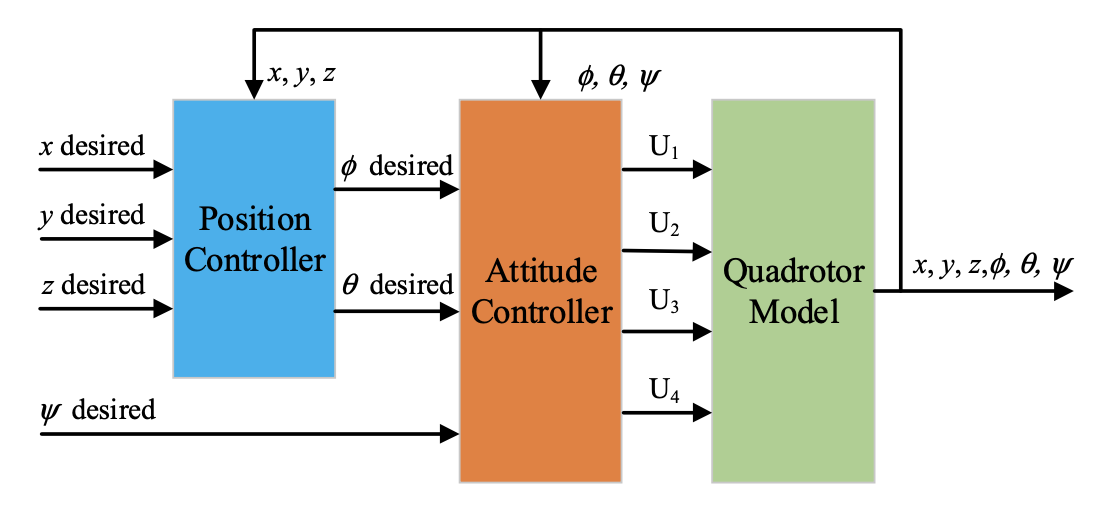
\includegraphics[width=0.8\textwidth]{gfx/quadControlSystem}
	\caption[Schema di controllo di un quadrirotore.]{Schema di controllo di un quadrirotore. L'anello più interno è responsabile del controllo di assetto (Attitude Controller), quello più esterno del controllo di posizione (Position Controller).}
	\label{fig:quadControlSystem}
\end{figure}

Le variabili considerate come input e output del modello sono rispettivamente quelle di controllo e di misura nello schema mostrato in Figura \ref{fig:quadControlSystem}. Come già spiegato, il quadrirotore è controllabile variando le velocità angolari dei quattro rotori ($\Omega_i$, $i = 1,2,3,4$). Tuttavia, le forze e i momenti generati dai rotori sono funzioni quadratiche delle velocità angolari, quindi considerare le velocità angolari come variabili di ingresso del modello comporterebbe sia una forte non linearità nelle equazioni (a causa della dipendenza quadratica), sia un forte accoppiamento tra gli ingressi e la risposta dei singoli assi (poiché le velocità angolari dei quattro rotori vengono sempre variate simultaneamente, indipendentemente dal grado di libertà da controllare). Per evitare queste difficoltà solitamente si considerano come ingressi i segnali di controllo $U_i$, $i = 1,2,3,4$ definiti nell'equazione \ref{defControls} del Capitolo \ref{ch:uav}. Siccome questi quattro segnali agiscono sulle quattro manovre principali del velivolo, si possono equivalentemente considerare gli angoli di Eulero e la forza di spinta come ingressi del sistema. Non è oggetto della tesi l'identificazione della dinamica dell'angolo di yaw, quindi si considerano in ingresso al modello la forza di spinta e gli angoli di roll e pitch. Infine, le variabili in uscita sono esattamente quelle di misura, cioè le coordinate del velivolo nello spazio.\\

Dal punto di vista implementativo, il controllore è un pacchetto \acs{ROS} contenente nodi (Python) di varia utilità. Alcuni nodi gestiscono l'algoritmo matematico di controllo, altri si occupano di presentare all'utente un'interfaccia grafica per controllare lo spostamento del drone. Come mostra Figura \ref{fig:drone_controller}, l'utente può effettuare le seguenti operazioni, che corrispondo a servizi \acs{ROS} nel codice sorgente:
\begin{itemize}
	\item \textbf{Take Off} fa decollare il drone all'altezza specificata e lo stabilizza (stato di hovering);
	\item \textbf{Go To Point} imposta il setpoint da raggiungere verso le coordinate desiderate (rispetto al sistema di riferimento specificato, che può essere sia quello a terra che quello solidale al velivolo);
	\item \textbf{Go Home} riporta il drone nelle componenti del piano XY iniziali in cui è avvenuto il decollo;
	\item \textbf{Land} fa atterrare il drone nel punto del piano XY dove si trova, disarmando i motori.
\end{itemize}

\begin{figure}[H]
	\centering
	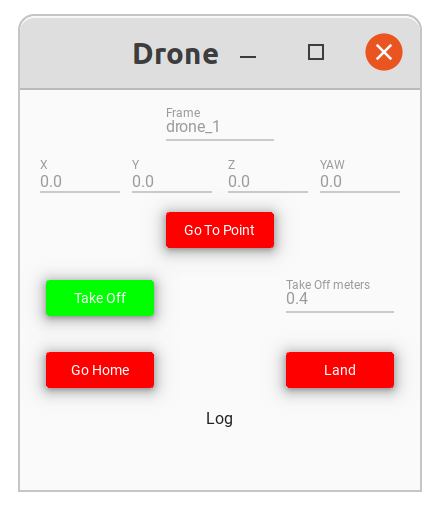
\includegraphics[width=0.4\textwidth]{gfx/ROS/drone_controller}
	\caption[Interfaccia grafica del controllore.]{Interfaccia grafica del controllore.}
	\label{fig:drone_controller}
\end{figure}

\subsection{Registrazione e Memorizzazione Dati}
I dati di interesse sono gli angoli di Eulero responsabili dei movimenti laterali del drone e la forza di spinta per quanto riguarda gli input e le coordinate di posizione per quanto riguarda gli output. Per registrare e memorizzare queste informazioni sono state aggiunte alcune righe di codice in alcuni nodi \acs{ROS} del controllore. In particolare, per la gestione dei dati sono state utilizzate le librerie NumPy \cite{numPy} e SciPy \cite{sciPy}.\\

Prima di tutto sono stati inizializzati sei array NumPy (tre per gli input e tre per gli output), poi sono stati riempiti all'interno del ciclo di controllo del drone utilizzando la funzione \emph{append()}, fornita dalla libreria NumPy. Il ciclo di controllo viene aggiornato con una frequenza di 100 Hz, quindi, al termine di una simulazione di volo ogni array sarà un segnale del tempo campionato con tempo di campionamento pari a 0.01 secondi. Il numero di campioni dipende dalla durata della simulazione e, ovviamente, tanto più è grande tanto più sarà precisa l'identificazione del modello. Ipotizzando che ogni volo registrato è durato in media due minuti, ogni segnale è caratterizzato da circa 12000 campioni. Sono state effettuate dieci simulazioni di volo in modo da poter identificare più modelli relativi a distinti insiemi di dati e confrontarli tra loro.\\

Per trasferire i dati registrati in MATLAB, dove poi avvengono i tre passi necessari per identificare e validare il sistema, si è fatto uso della funzione \emph{savemat()} \cite{savemat} della libreria input-output di SciPy (\emph{scipy.io}).

% ------------------------------ SISO ------------------------------

\section{Identificazione di Modelli SISO}
L'obiettivo di questa sezione è quello di identificare tre funzioni di trasferimento tempo continue, nel dominio di Laplace, che descrivano le dinamiche del quadrirotore sugli assi principali. Infatti, il quadrirotore mostra un buon grado di disaccoppiamento, cioè l'azione su uno dei segnali di controllo influisce quasi esclusivamente sul corrispondente grado di libertà \cite{idEsempio} \cite{decoupledDynamics}.

\subsection{Rappresentazione di Sistemi Lineari}
Nel campo dell'analisi di sistemi, un sistema dinamico \acs{SISO}, lineare e tempo-invariante - \ac{LTI} - è descritto da un'equazione differenziale lineare a coefficienti costanti in $u(t)$ e $y(t)$ (rispettivamente ingresso e uscita). Assumendo condizioni iniziali nulle e applicando la trasformata di Laplace, si ottiene un'equazione algebrica del tipo:
\[ Y(s) = W(s)U(s) \]
dove $U(s)$ e $Y(s)$ sono i segnali di ingresso e uscita trasformati e $W(s)$ è la funzione di trasferimento che li lega. Inoltre, una equazione differenziale lineare a coefficienti costanti genera sempre una funzione di trasferimento razionale fratta, cioè esprimibile come il rapporto di due polinomi.

\pagebreak

\subsection{Funzione di Trasferimento angolo di Rollio e posizione lungo Y}
I dati utilizzati per identificare la dinamica del velivolo lungo l'asse Y sono il segnale che descrive le variazioni dell'angolo di rollio (input) e il segnale che descrive le variazioni di posizione lungo lo stesso asse (output). Entrambi i segnali si presentano già a media nulla\footnote{Il processo che elimina la media di un segnale e lo rende a media nulla viene denominato detrending e consente di rimuovere gli effetti del valor medio per mostrare solo le differenze significative. Consente quindi di identificare in modo più preciso l'andamento del segnale.}, quindi l'unica operazione di preprocessing effettuata è stata quella di considerare uno specifico intervallo temporale (dove il segnale è significativo). I segnali utilizzati sono mostrati in Figura \ref{fig:ry_input}. Il segnale di input, relativo all'angolo di rollio, mostra una brusca variazione prima di assestarsi a zero. Questo accade perché al termine della simulazione di volo, quando si fa atterrare il drone, il controllore cerca di stabilizzare il drone nel punto del piano XY dove si trova. Ma non appena il drone inizia il processo di atterraggio, il controllore smette di inviare controlli relativi all'assetto del velivolo e l'angolo di rollio (in questo caso) rimane nullo fino al termine della simulazione.

\begin{figure}[H]
	\centering
	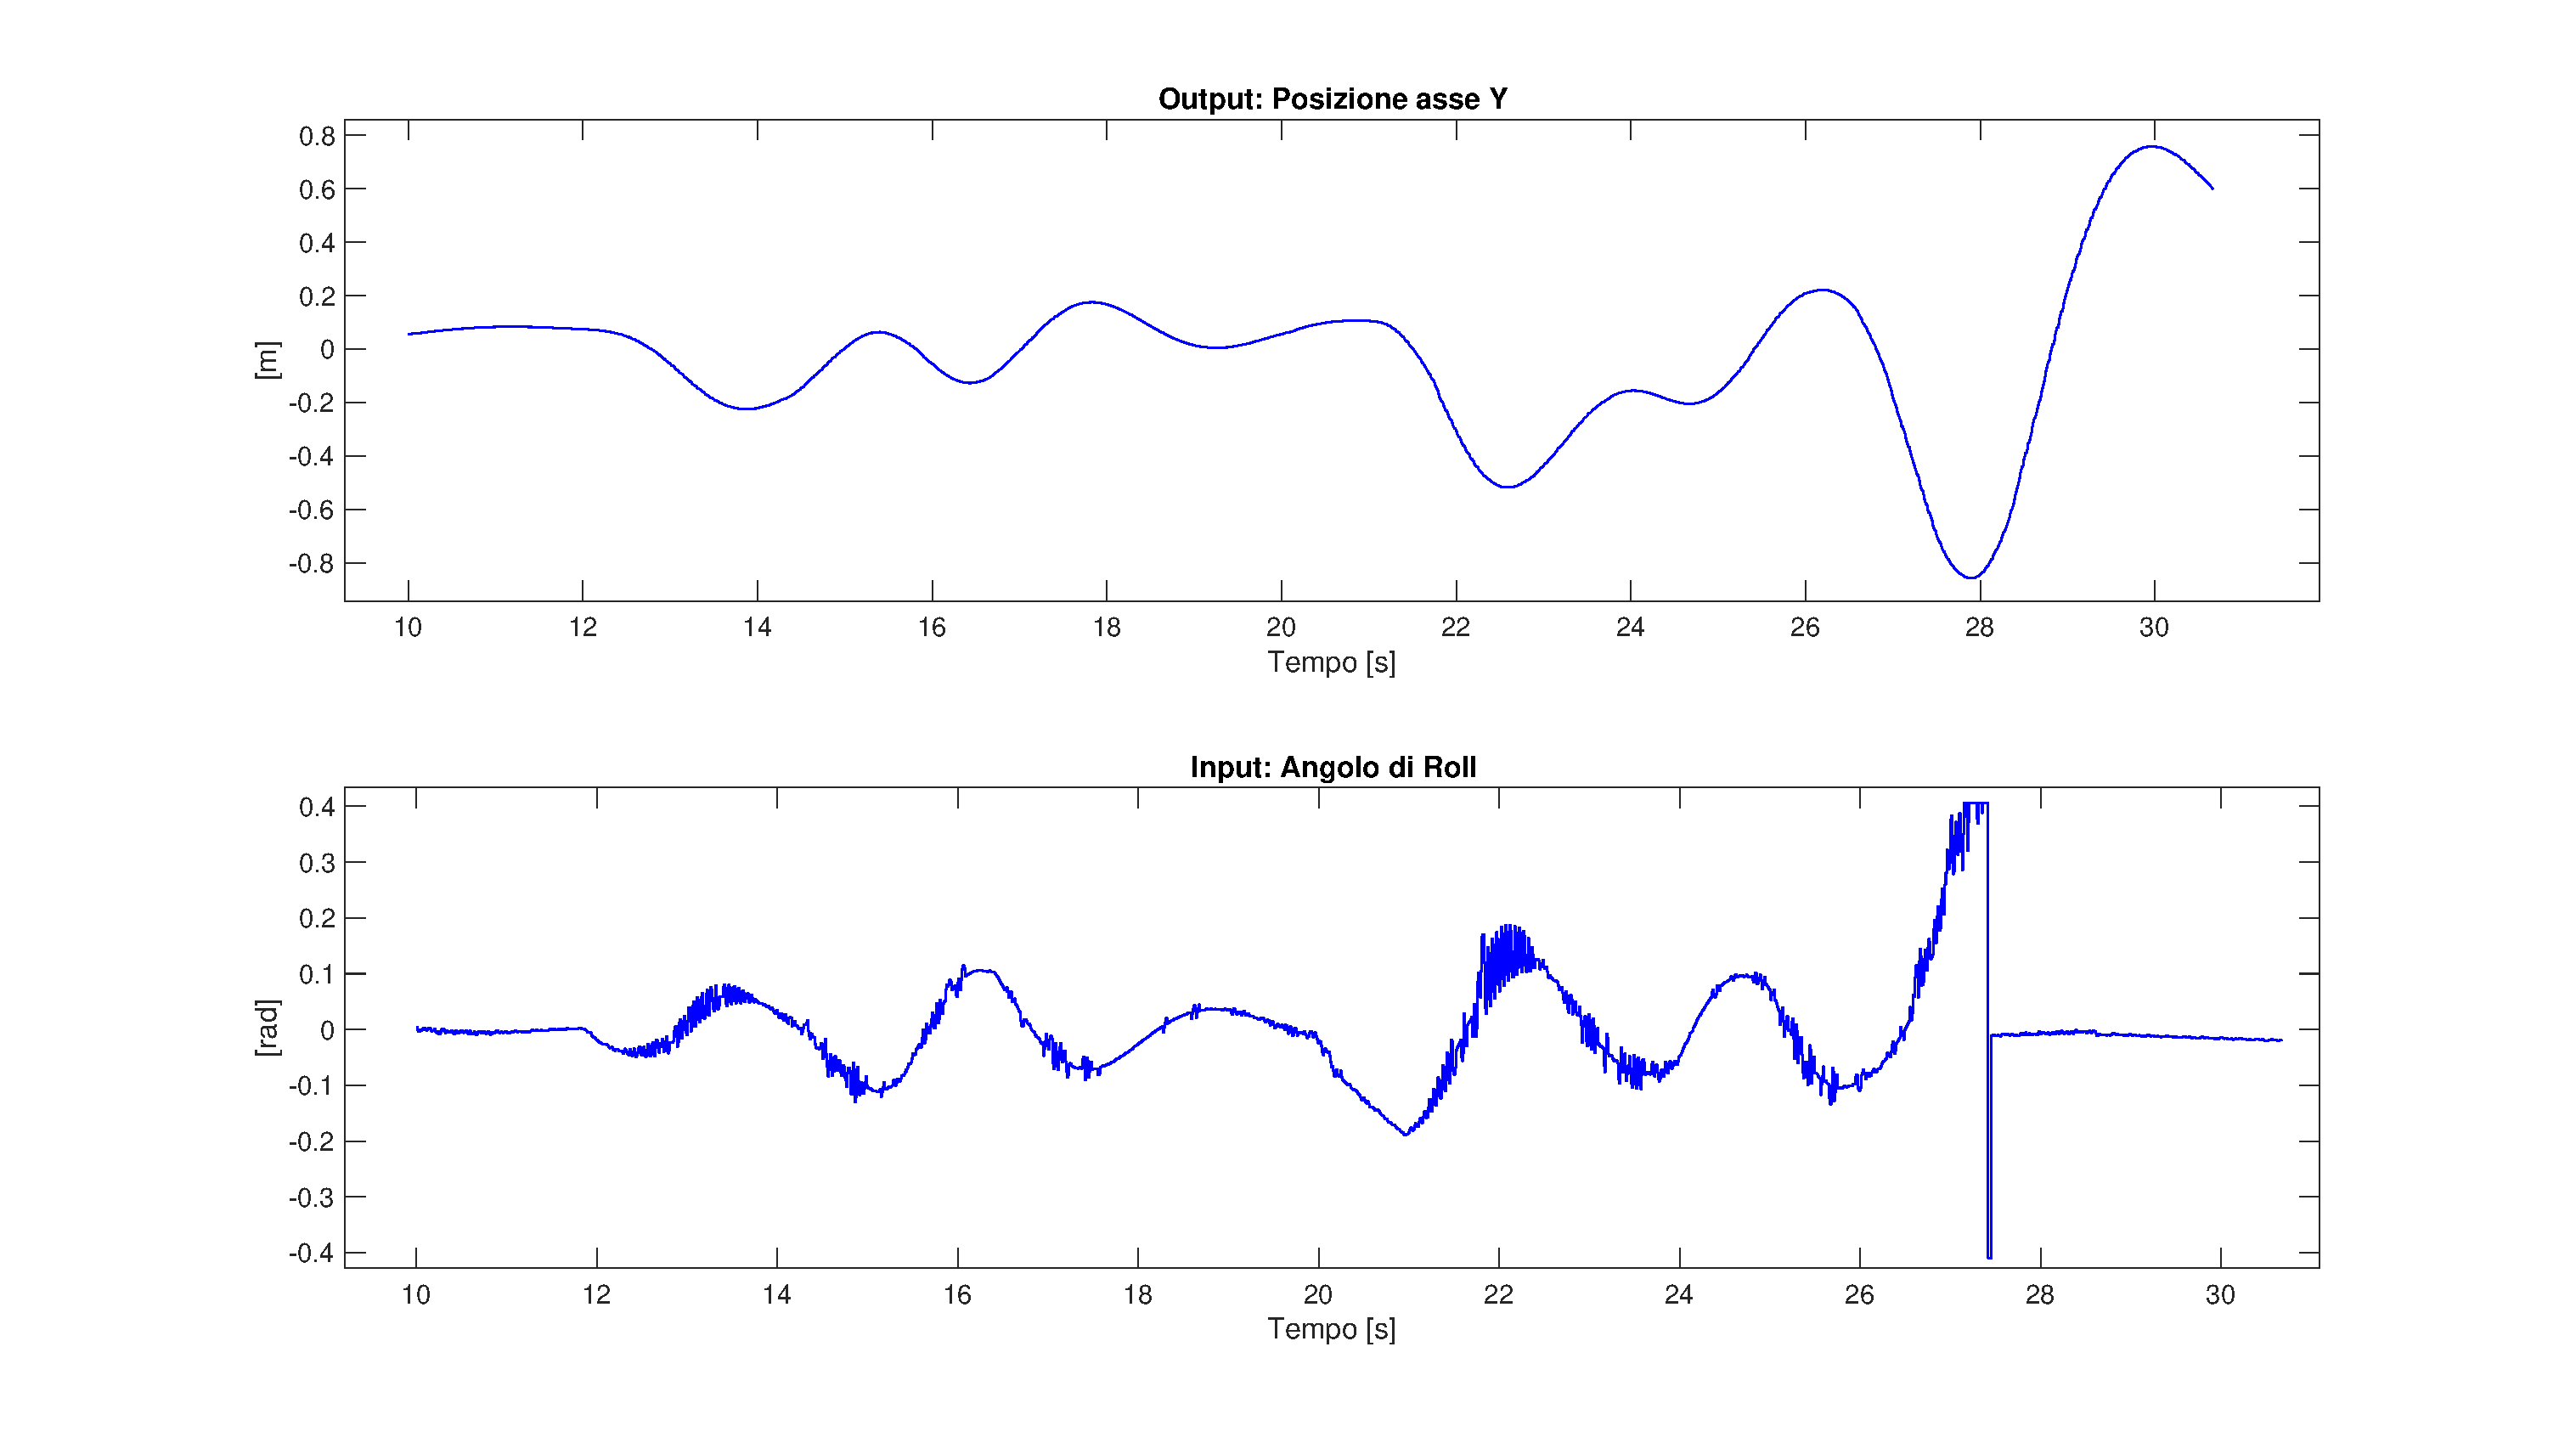
\includegraphics[width=1\textwidth]{gfx/SysId/ryinput}
	\caption[Dati input-output per identificare la dinamica del rollio.]{Dati input-output per identificare la dinamica del rollio. Input: variazione dell'angolo di rollio nel tempo. Output: variazione della posizione lungo l'asse Y nel tempo.}
	\label{fig:ry_input}
\end{figure}

La funzione di trasferimento identificata che lega l'angolo di rollio (roll) allo spostamento del velivolo lungo l'asse Y è definita nell'equazione \ref{fdtY}.

\begin{equation}
	W_Y(s) = \frac{-1.022s^2 + 0.6857s + 1.873}{s^3 + 0.008794s^2 + 1.456s + 0.1566}
	= \frac{-1.022(s-1.73)(s+1.059)}{(s+0.1068)(s-0.0490\pm j1.2098)}
	\label{fdtY}
\end{equation}

Si tratta di un sistema lineare tempo continuo del terzo ordine con un polo reale e due poli complessi e coniugati.\\

Completata la fase di identificazione, si passa alla terza e ultima fase, cioè la validazione del sistema. La funzione \emph{compare()} \cite{compare} mostra una buona compatibilità del modello identificato con quello reale, come mostra Figura \ref{fig:ry_model}. Il \acs{NRMSE} risulta in un 71.3\% di compatibilità.

\begin{figure}[H]
	\centering
	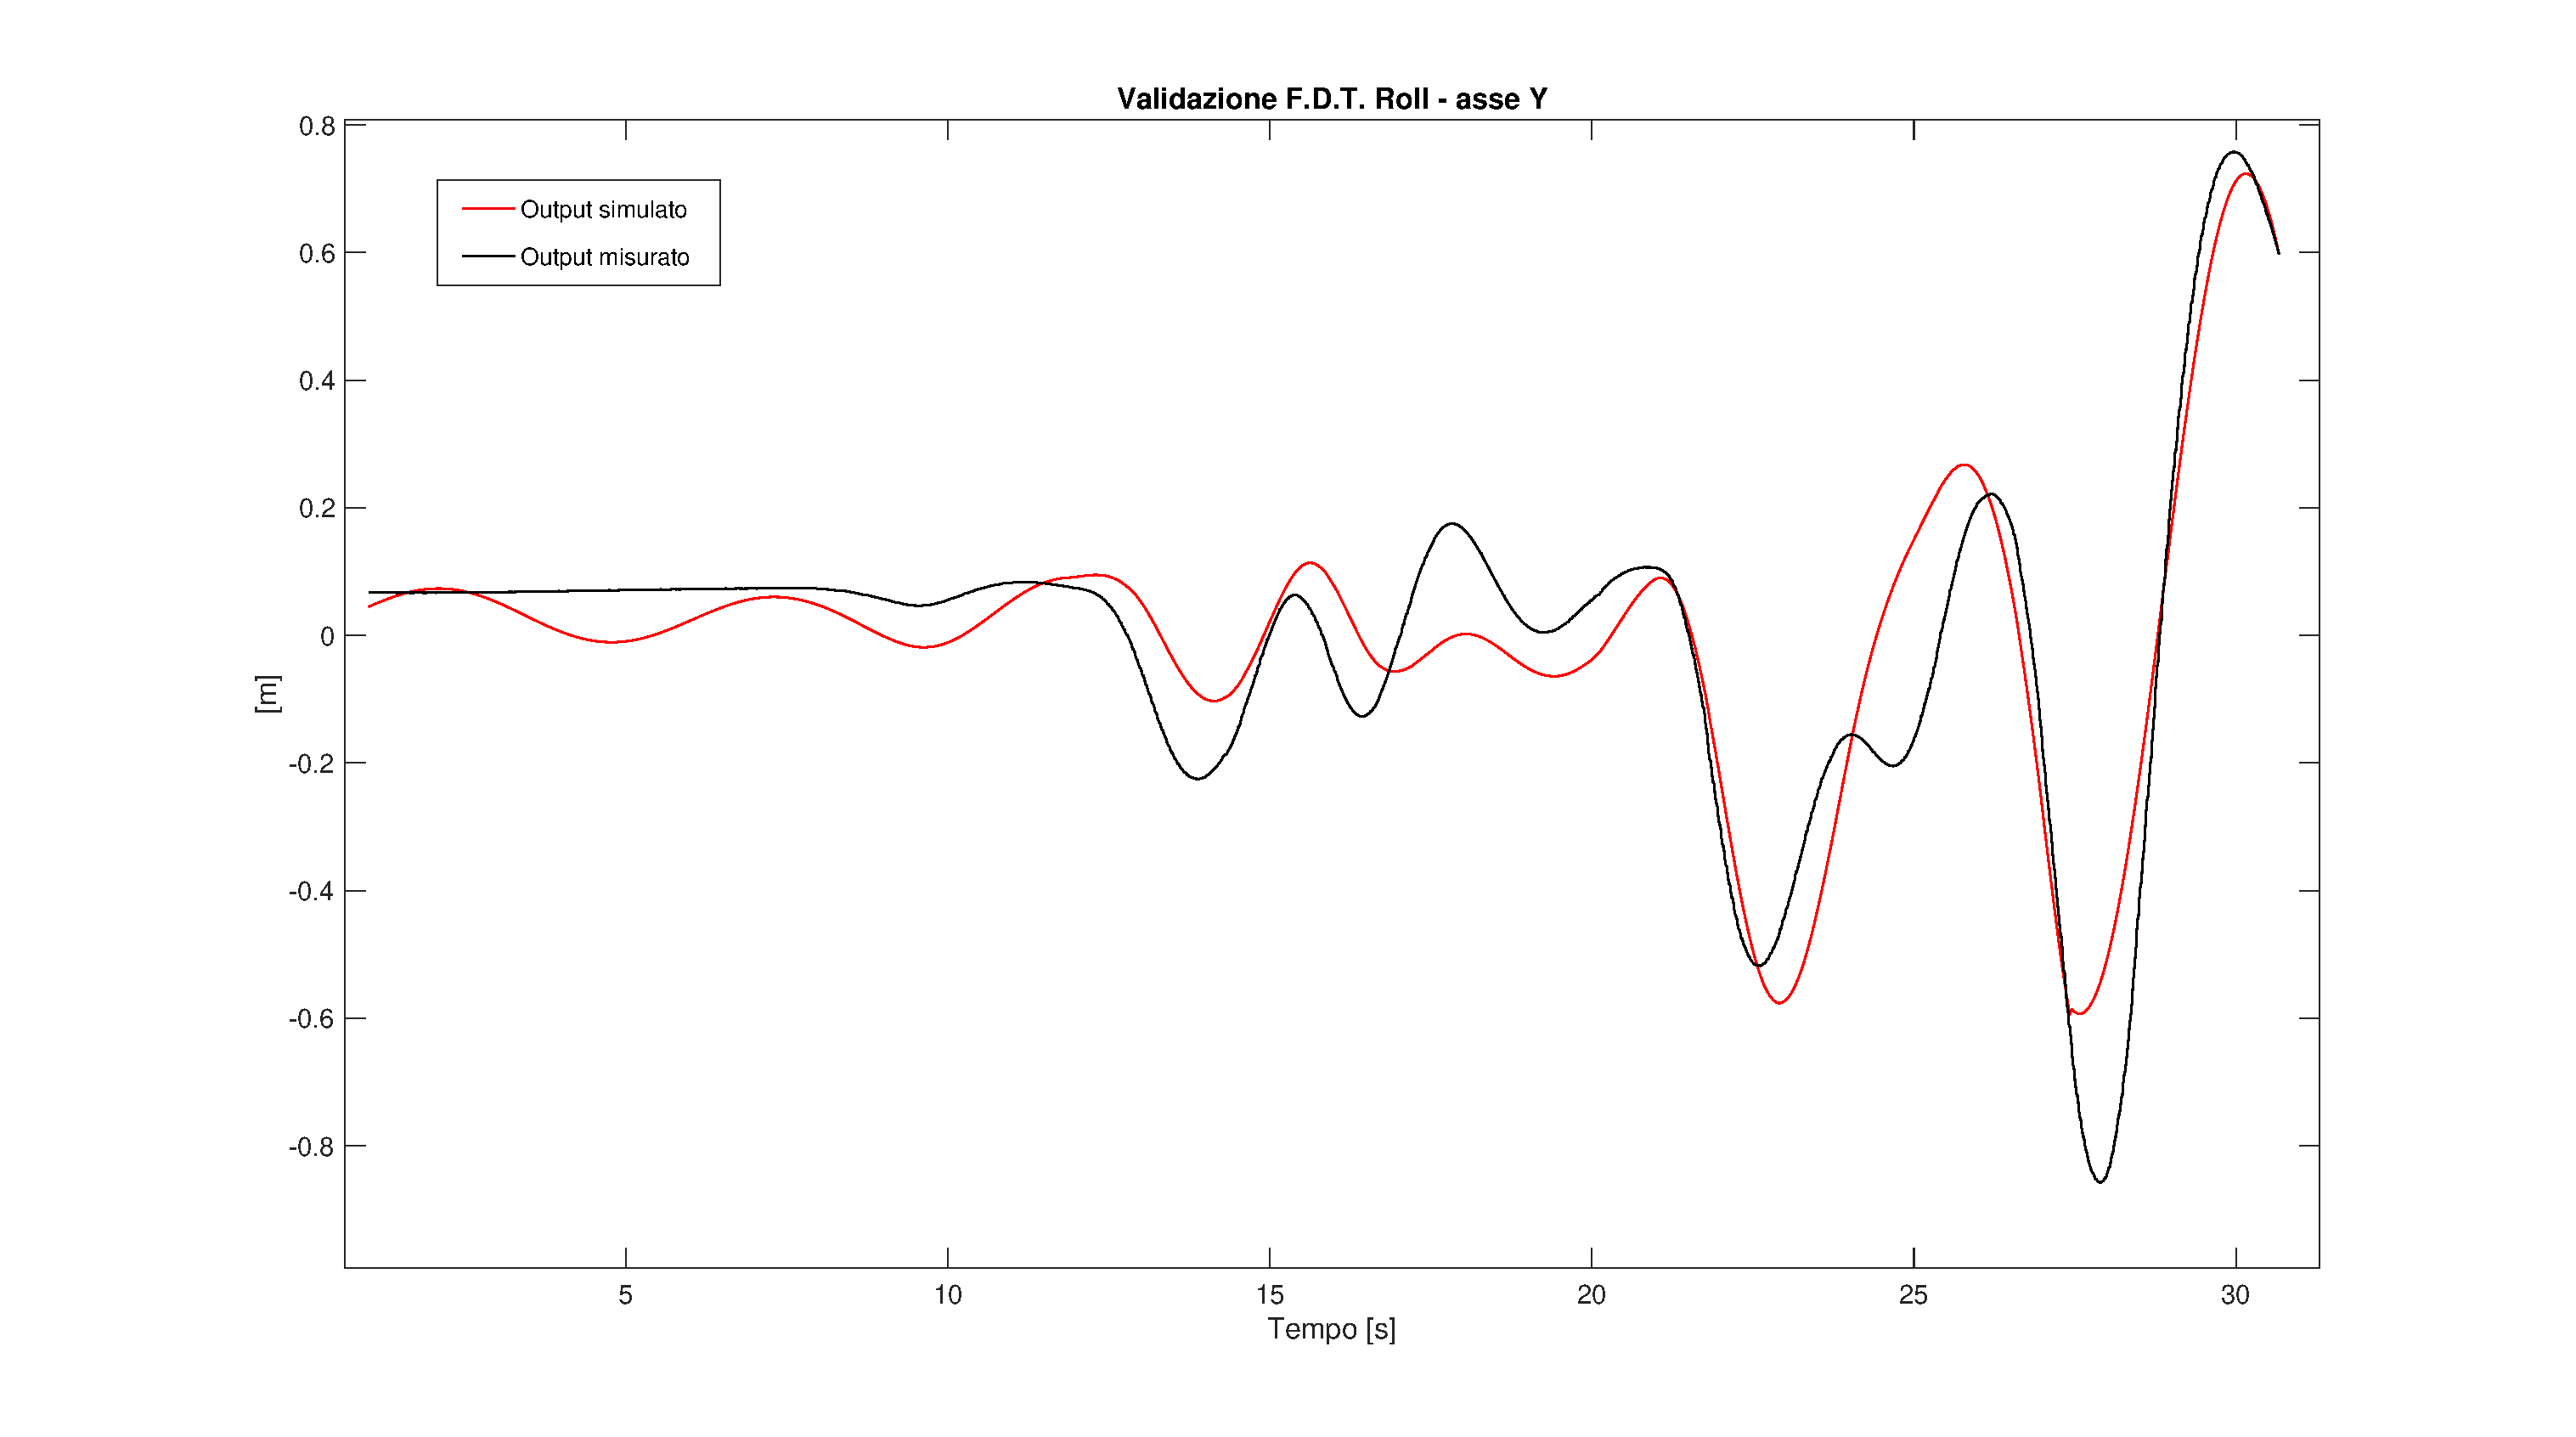
\includegraphics[width=1\textwidth]{gfx/SysId/rymodel}
	\caption[Validazione F.D.T. Rollio e posizione lungo Y.]{Validazione F.D.T. tra rollio e posizione lungo Y.}
	\label{fig:ry_model}
\end{figure}

\subsection{Funzione di Trasferimento angolo di Beccheggio e posizione lungo X}
I dati utilizzati per identificare la dinamica del velivolo lungo l'asse X sono il segnale che descrive le variazioni dell'angolo di beccheggio (input) e il segnale che descrive le variazioni di posizione lungo lo stesso asse (output). Anche qui, entrambi i segnali si presentano già a media nulla, quindi l'unica operazione di preprocessing effettuata è stata quella di considerare uno specifico intervallo temporale (dove il segnale è significativo). I segnali utilizzati sono mostrati in Figura \ref{fig:px_input}.

\begin{figure}[H]
	\centering
	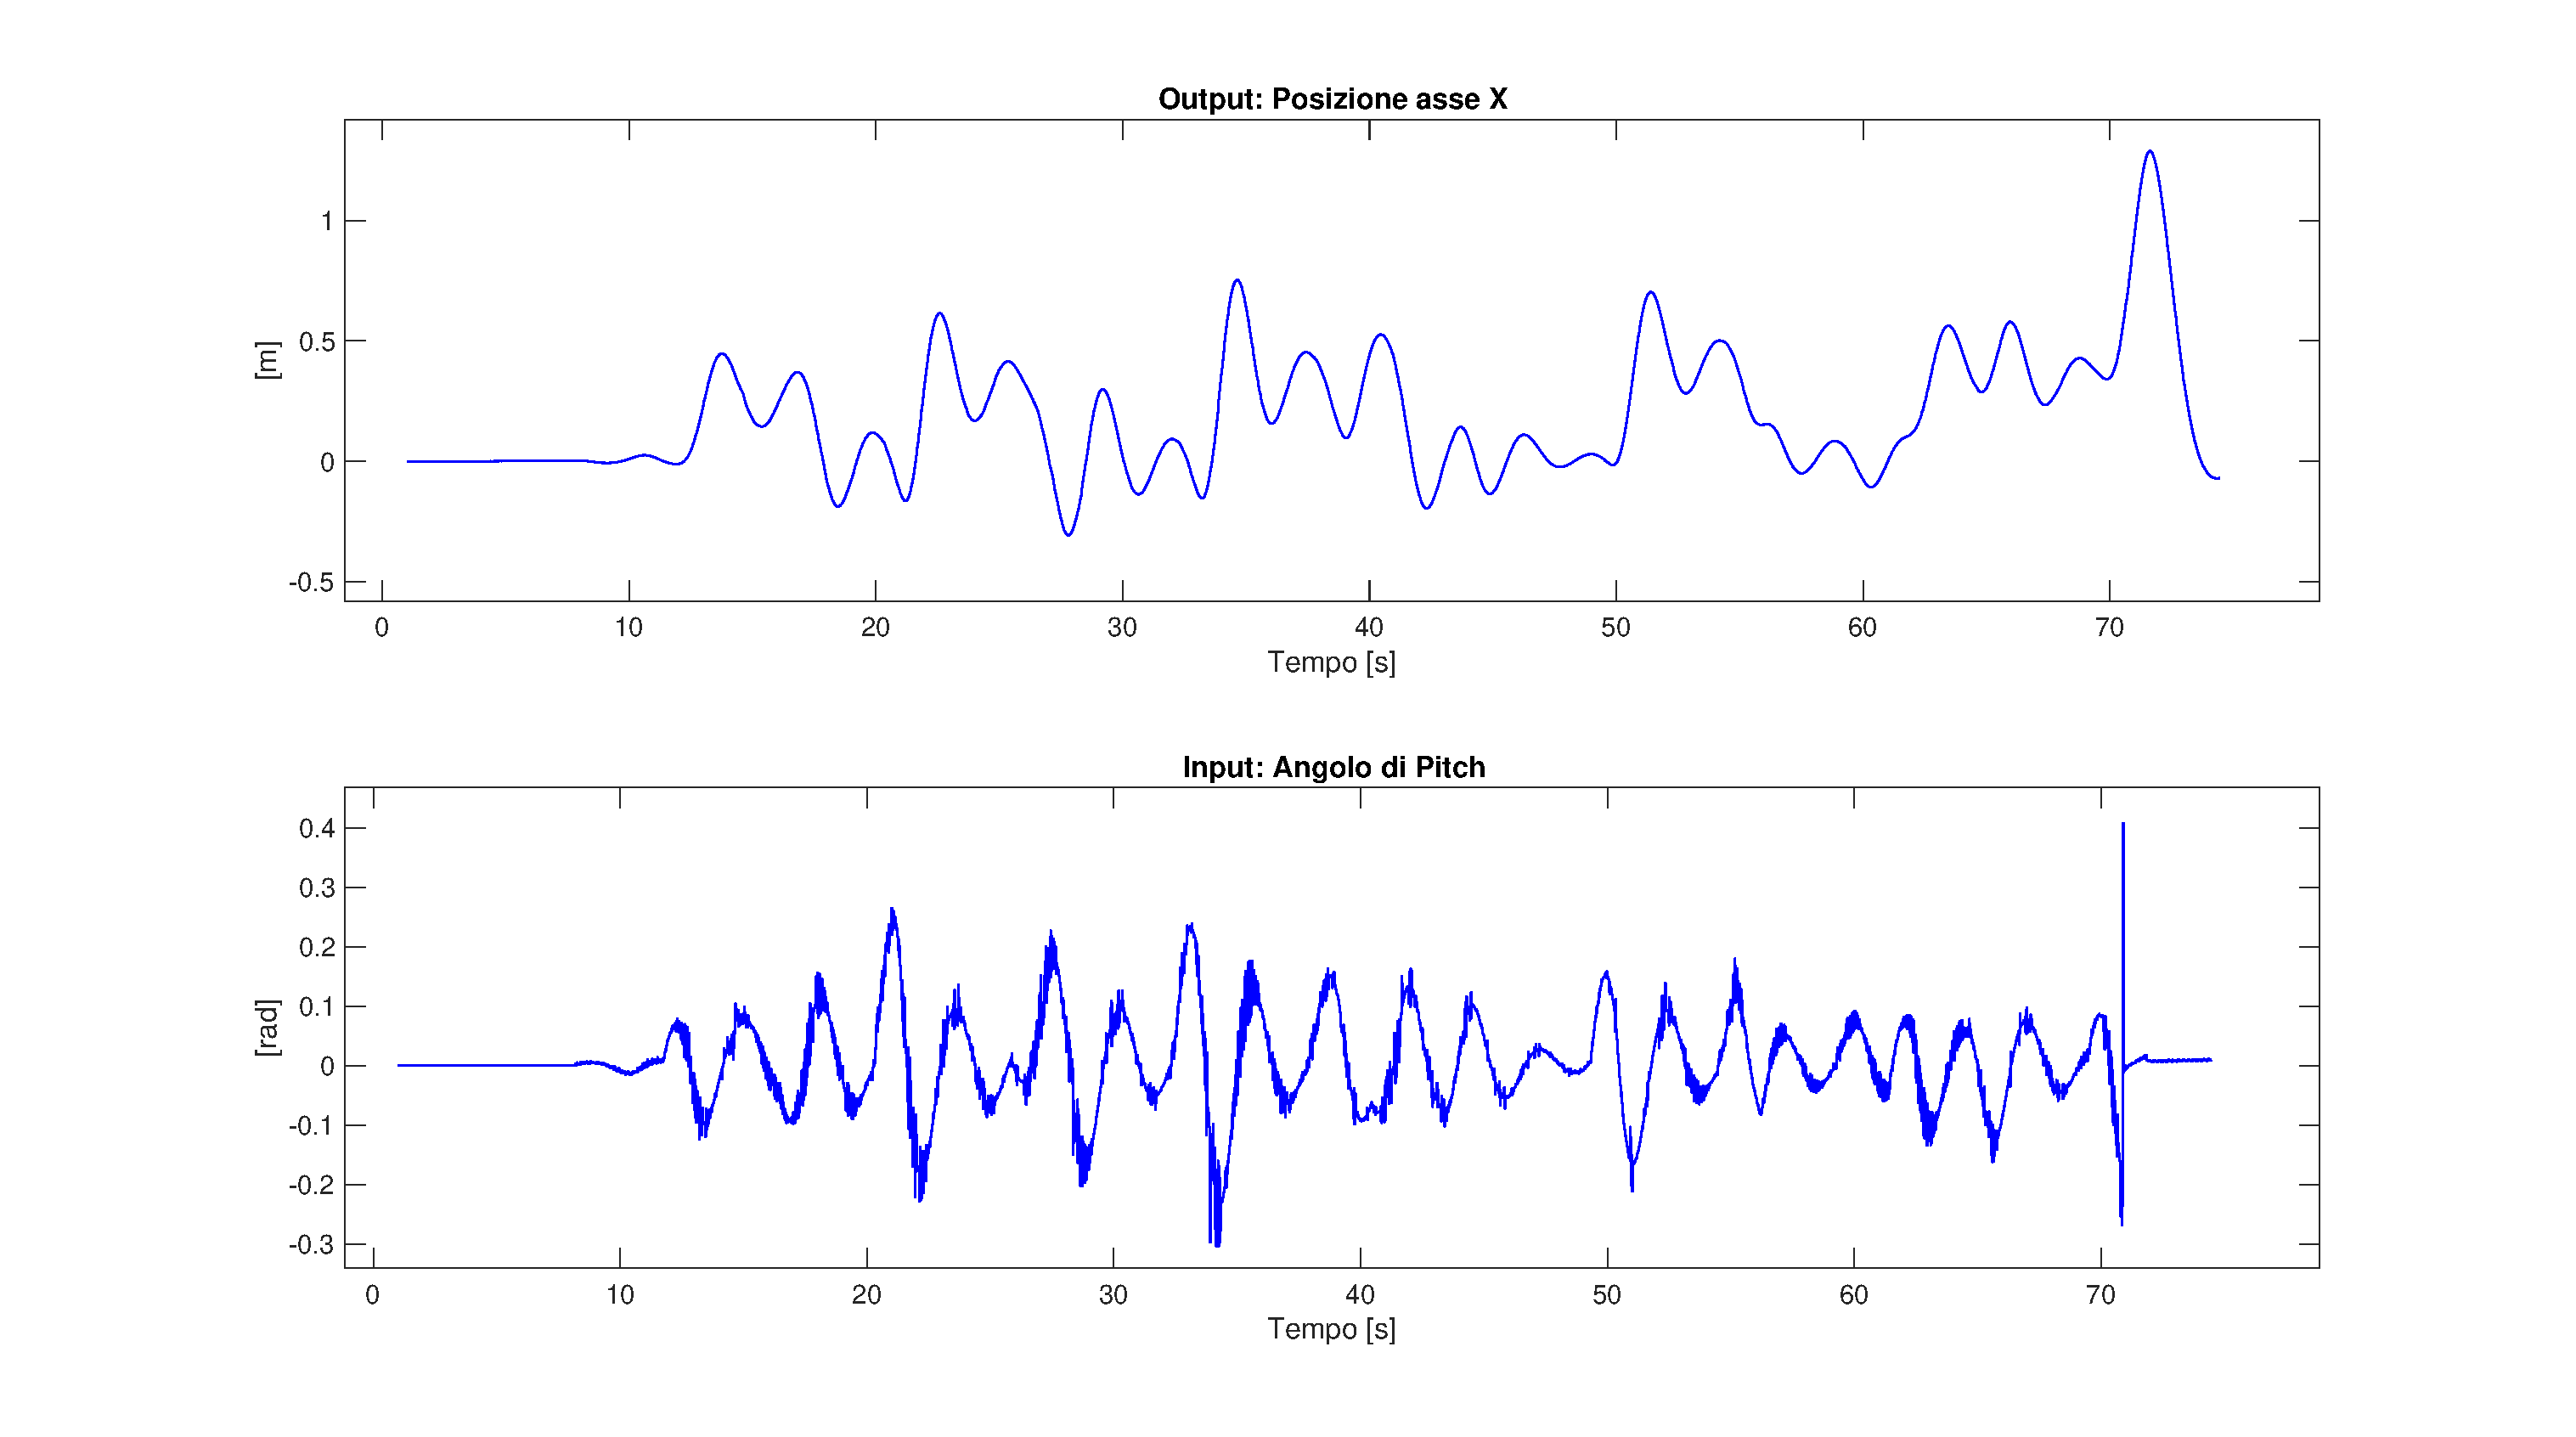
\includegraphics[width=1\textwidth]{gfx/SysId/pxinput}
	\caption[Dati input-output per identificare la dinamica del beccheggio.]{Dati input-output per identificare la dinamica del beccheggio. Input: variazione dell'angolo di beccheggio nel tempo. Output: variazione della posizione lungo l'asse X nel tempo.}
	\label{fig:px_input}
\end{figure}

La funzione di trasferimento identificata che lega l'angolo di beccheggio (pitch) allo spostamento del velivolo lungo l'asse X è definita nell'equazione \ref{fdtX}.

\begin{equation}
	W_X(s) = \frac{-3.224s^2 + 3.491s + 1.71}{s^3 + 1.16s^2 + 0.1916s + 0.1929}
	= \frac{-3.224(s-1.449)(s+0.3661)}{(s+1.14)(s-0.0714\pm j1.0995)}
	\label{fdtX}
\end{equation}

Anche in questo caso (non sorprendentemente per la simmetria del quadrirotore rispetto ai movimenti lungo Y e X) si ottiene un sistema lineare tempo continuo del terzo ordine con un polo reale e due poli complessi e coniugati.\\

Per quanto riguarda la validazione, la funzione \emph{compare()} \cite{compare} mostra ancora una buona compatibilità del modello identificato con quello reale, come mostra Figura \ref{fig:px_model}. Il \acs{NRMSE} risulta in un 69.7\% di compatibilità.

\begin{figure}[H]
	\centering
	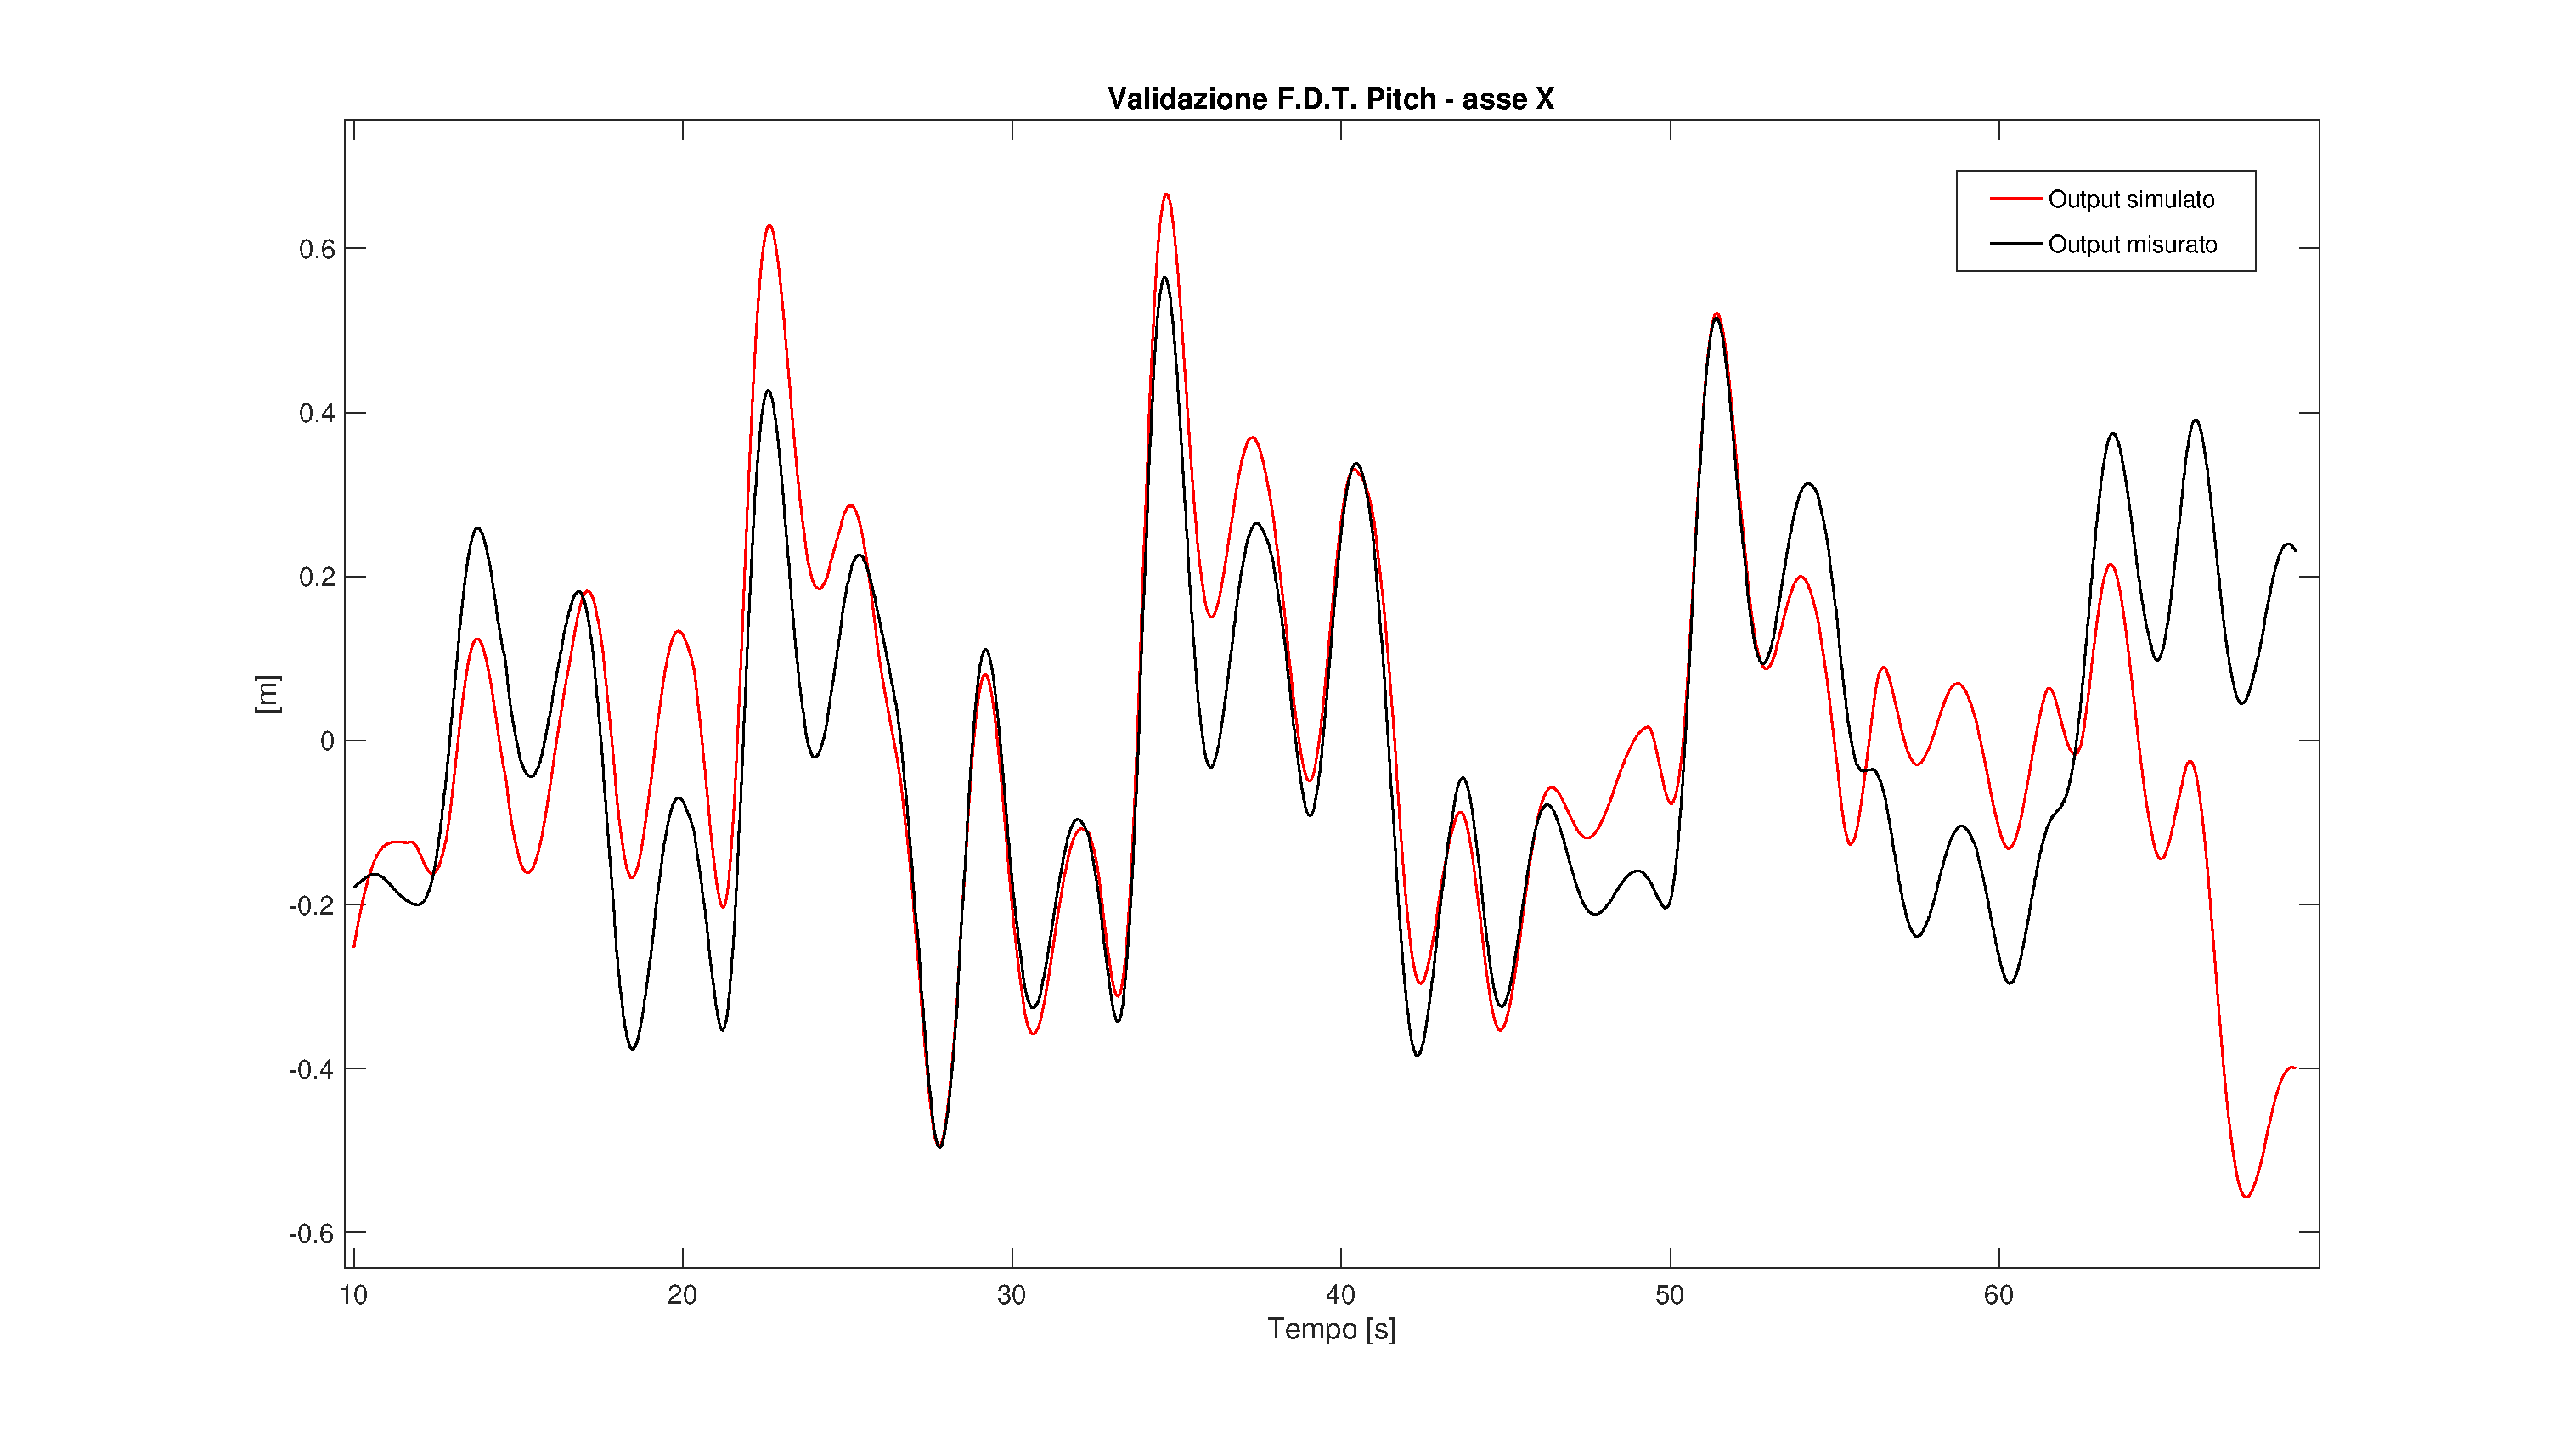
\includegraphics[width=1\textwidth]{gfx/SysId/pxmodel}
	\caption[Validazione F.D.T. Beccheggio e posizione lungo X.]{Validazione F.D.T. tra beccheggio e posizione lungo X.}
	\label{fig:px_model}
\end{figure}

\subsection{Funzione di Trasferimento forza di Spinta e posizione lungo Z}
I dati utilizzati per identificare la dinamica del velivolo lungo l'asse Z sono il segnale che descrive le variazioni della forza di spinta (input) e il segnale che descrive le variazioni di posizione lungo lo stesso asse (output). Il drone subito dopo il decollo entra in stato di hovering, cioè rimane fisso sull'origine del piano XY ma ad una certa quota lungo l'asse Z. Questo significa che, a differenza dei due casi precedenti, in questo caso i segnali input-output non sono a media nulla. Pertanto, nel preprocessing si rendono entrambi a media nulla, come mostra Figura \ref{fig:tz_input}.\\

Il segnale di ingresso contenente le varie spinte applicate nel tempo è caratterizzato da una serie di gradini, di diversa ampiezza, in modo da evidenziare in maniera marcata il comportamento del sistema. Si è cercato di fare la stessa cosa per gli ingressi utilizzati nei casi precedenti, ma il meccanismo di stabilizzazione è risultato meno efficiente per spostamenti sul piano XY (rispetto a spostamenti lungo l'asse Z), ed è per questo che i segnali sono sicuramente più complicati da interpretare.

\begin{figure}[H]
	\centering
	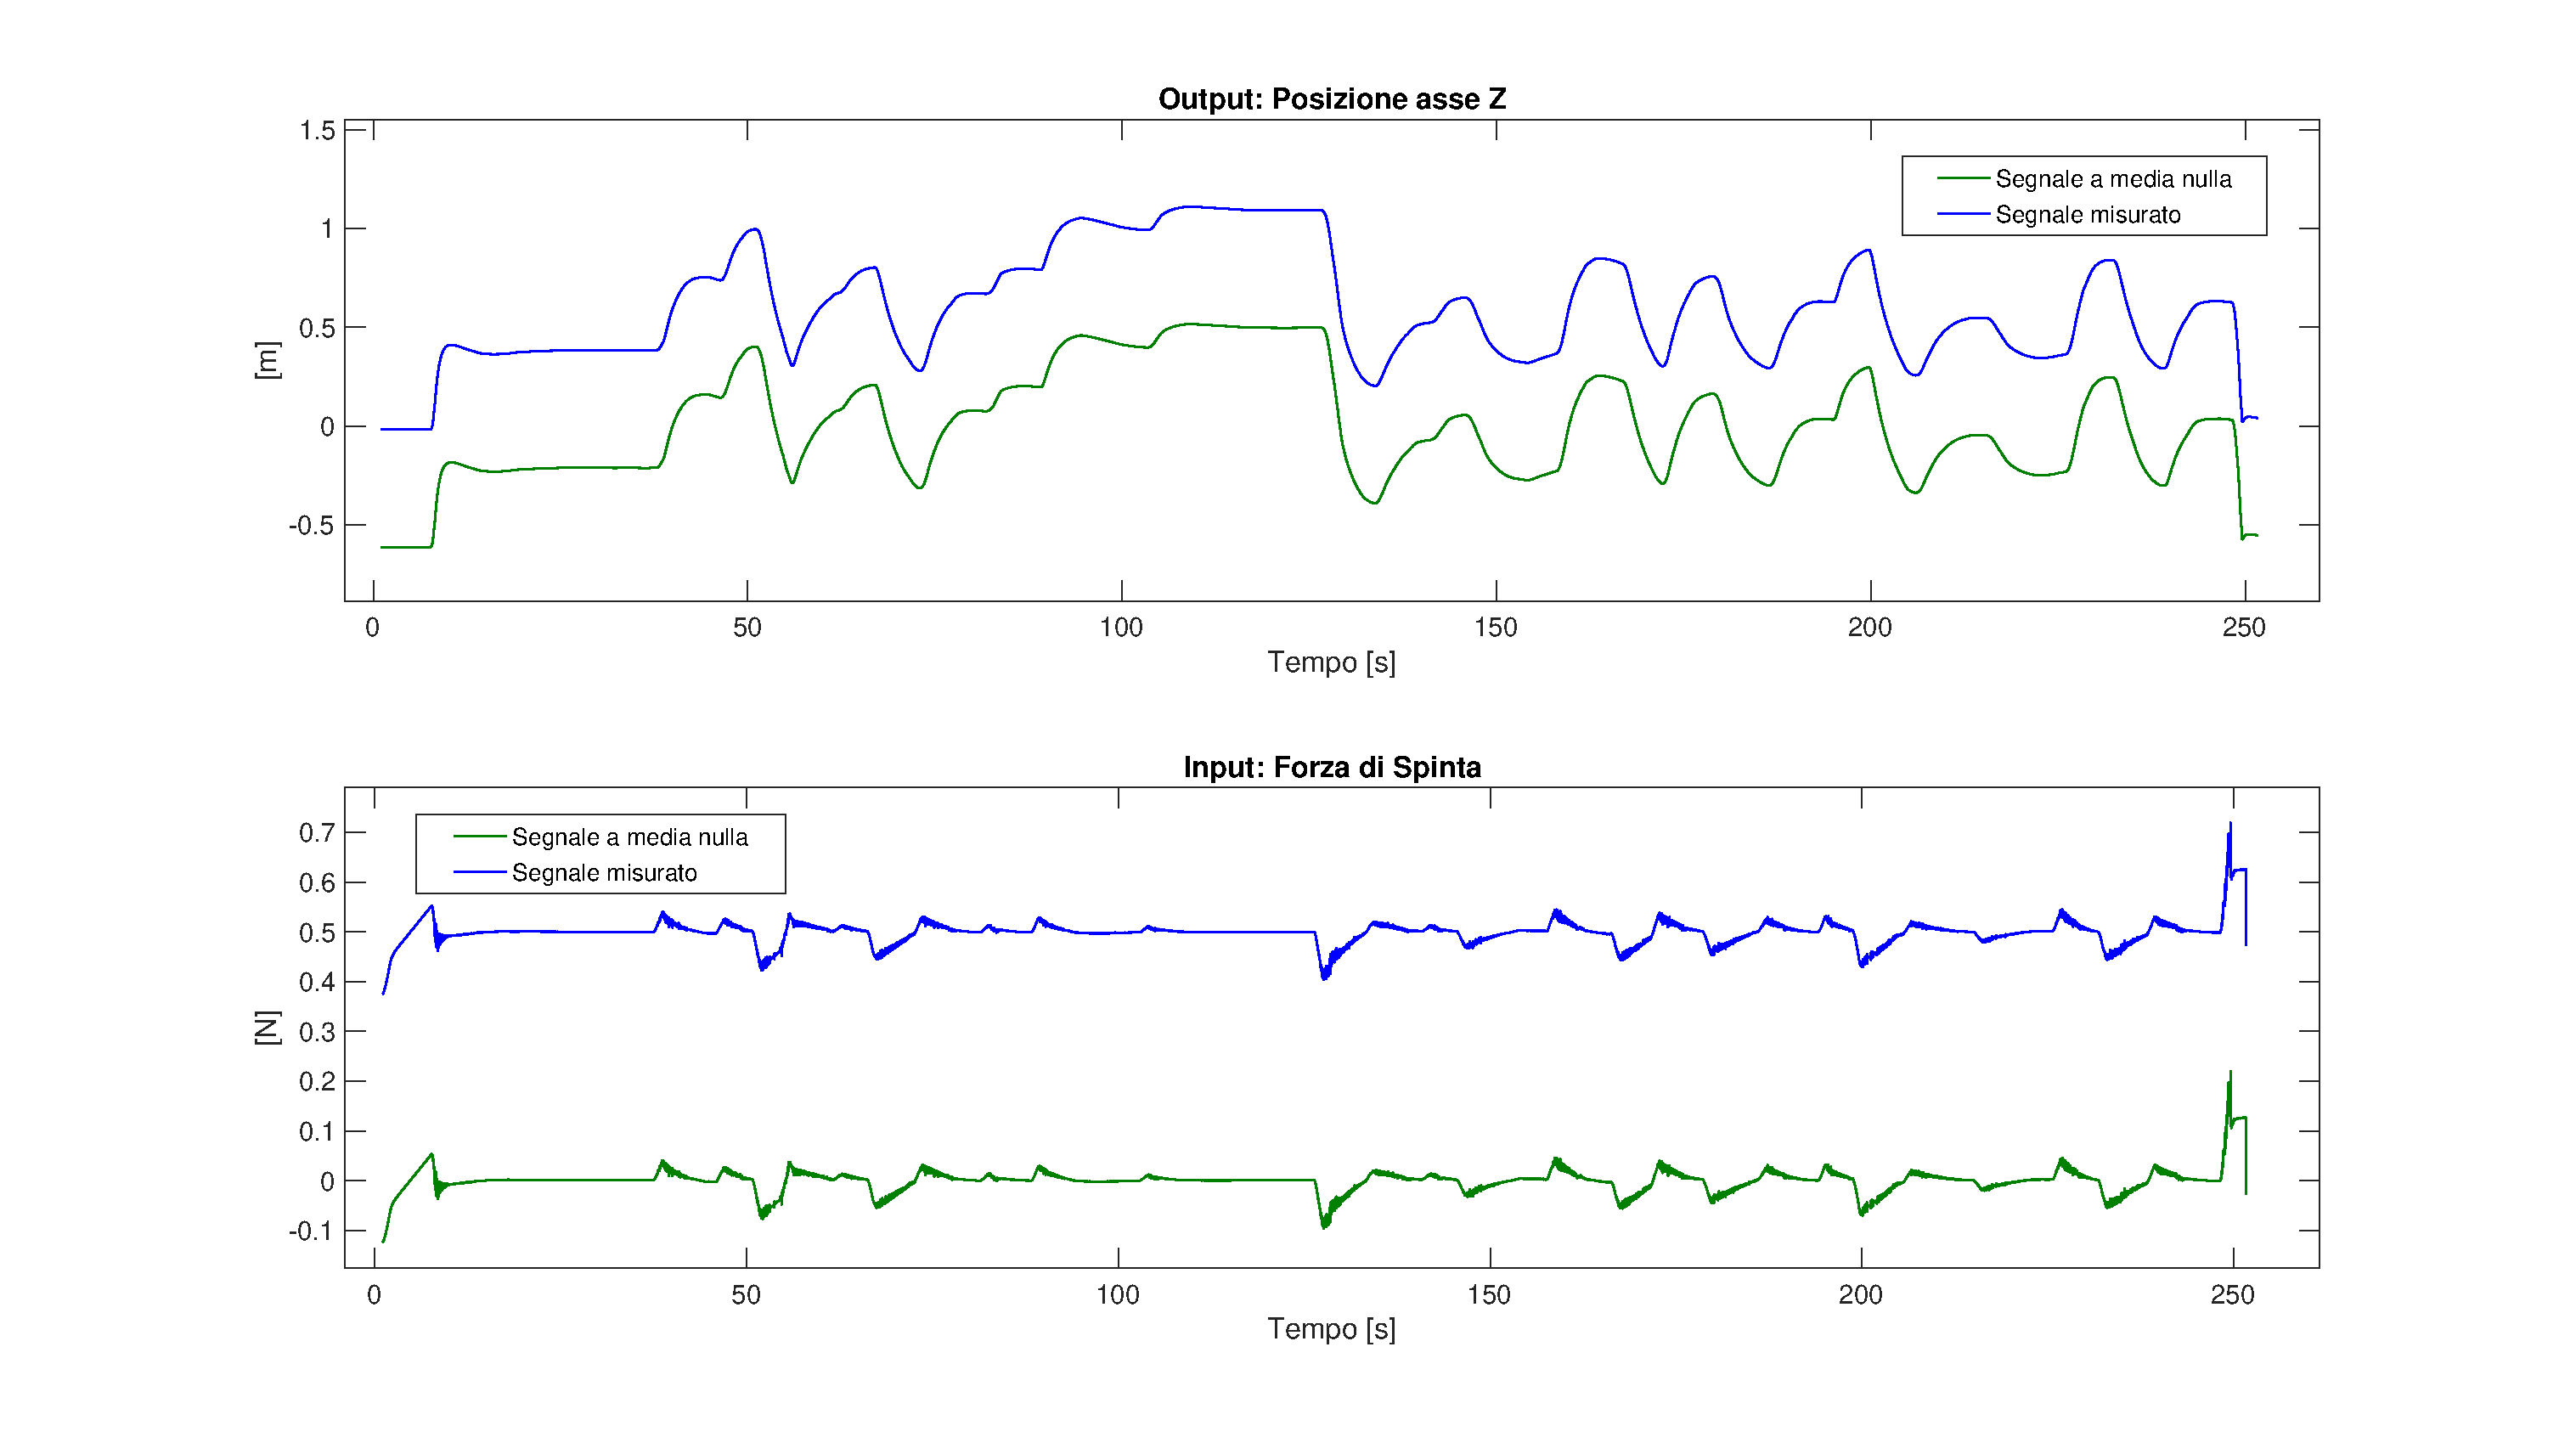
\includegraphics[width=1\textwidth]{gfx/SysId/tzinput}
	\caption[Dati input-output per identificare la dinamica della spinta.]{Dati input-output per identificare la dinamica della spinta. Input: forza di spinta applicata nel tempo. Output: variazione della posizione lungo l'asse Z nel tempo.}
	\label{fig:tz_input}
\end{figure}

La funzione di trasferimento identificata che lega la forza di spinta allo spostamento del velivolo lungo l'asse Z è mostrata nell'equazione \ref{fdtZ}.

\begin{equation}
	W_Z(s) = \frac{-144.02s^2 + 97.89s + 25.18}{s^3 + 39.98s^2 + 12.35s + 0.7329}
	= \frac{-144.02(s-0.8787)(s+0.199)}{(s+39.67)(s+0.231)(s+0.07999)}
	\label{fdtZ}
\end{equation}

Si ottiene ancora un sistema lineare tempo continuo del terzo ordine, ma con tre poli reali negativi.\\

Passando alla validazione, la funzione \emph{compare()} \cite{compare} mostra un'ottima compatibilità del modello identificato con quello reale, come mostra Figura \ref{fig:tz_model}. Il \acs{NRMSE} risulta in un 78.4\% di compatibilità.

\begin{figure}[H]
	\centering
	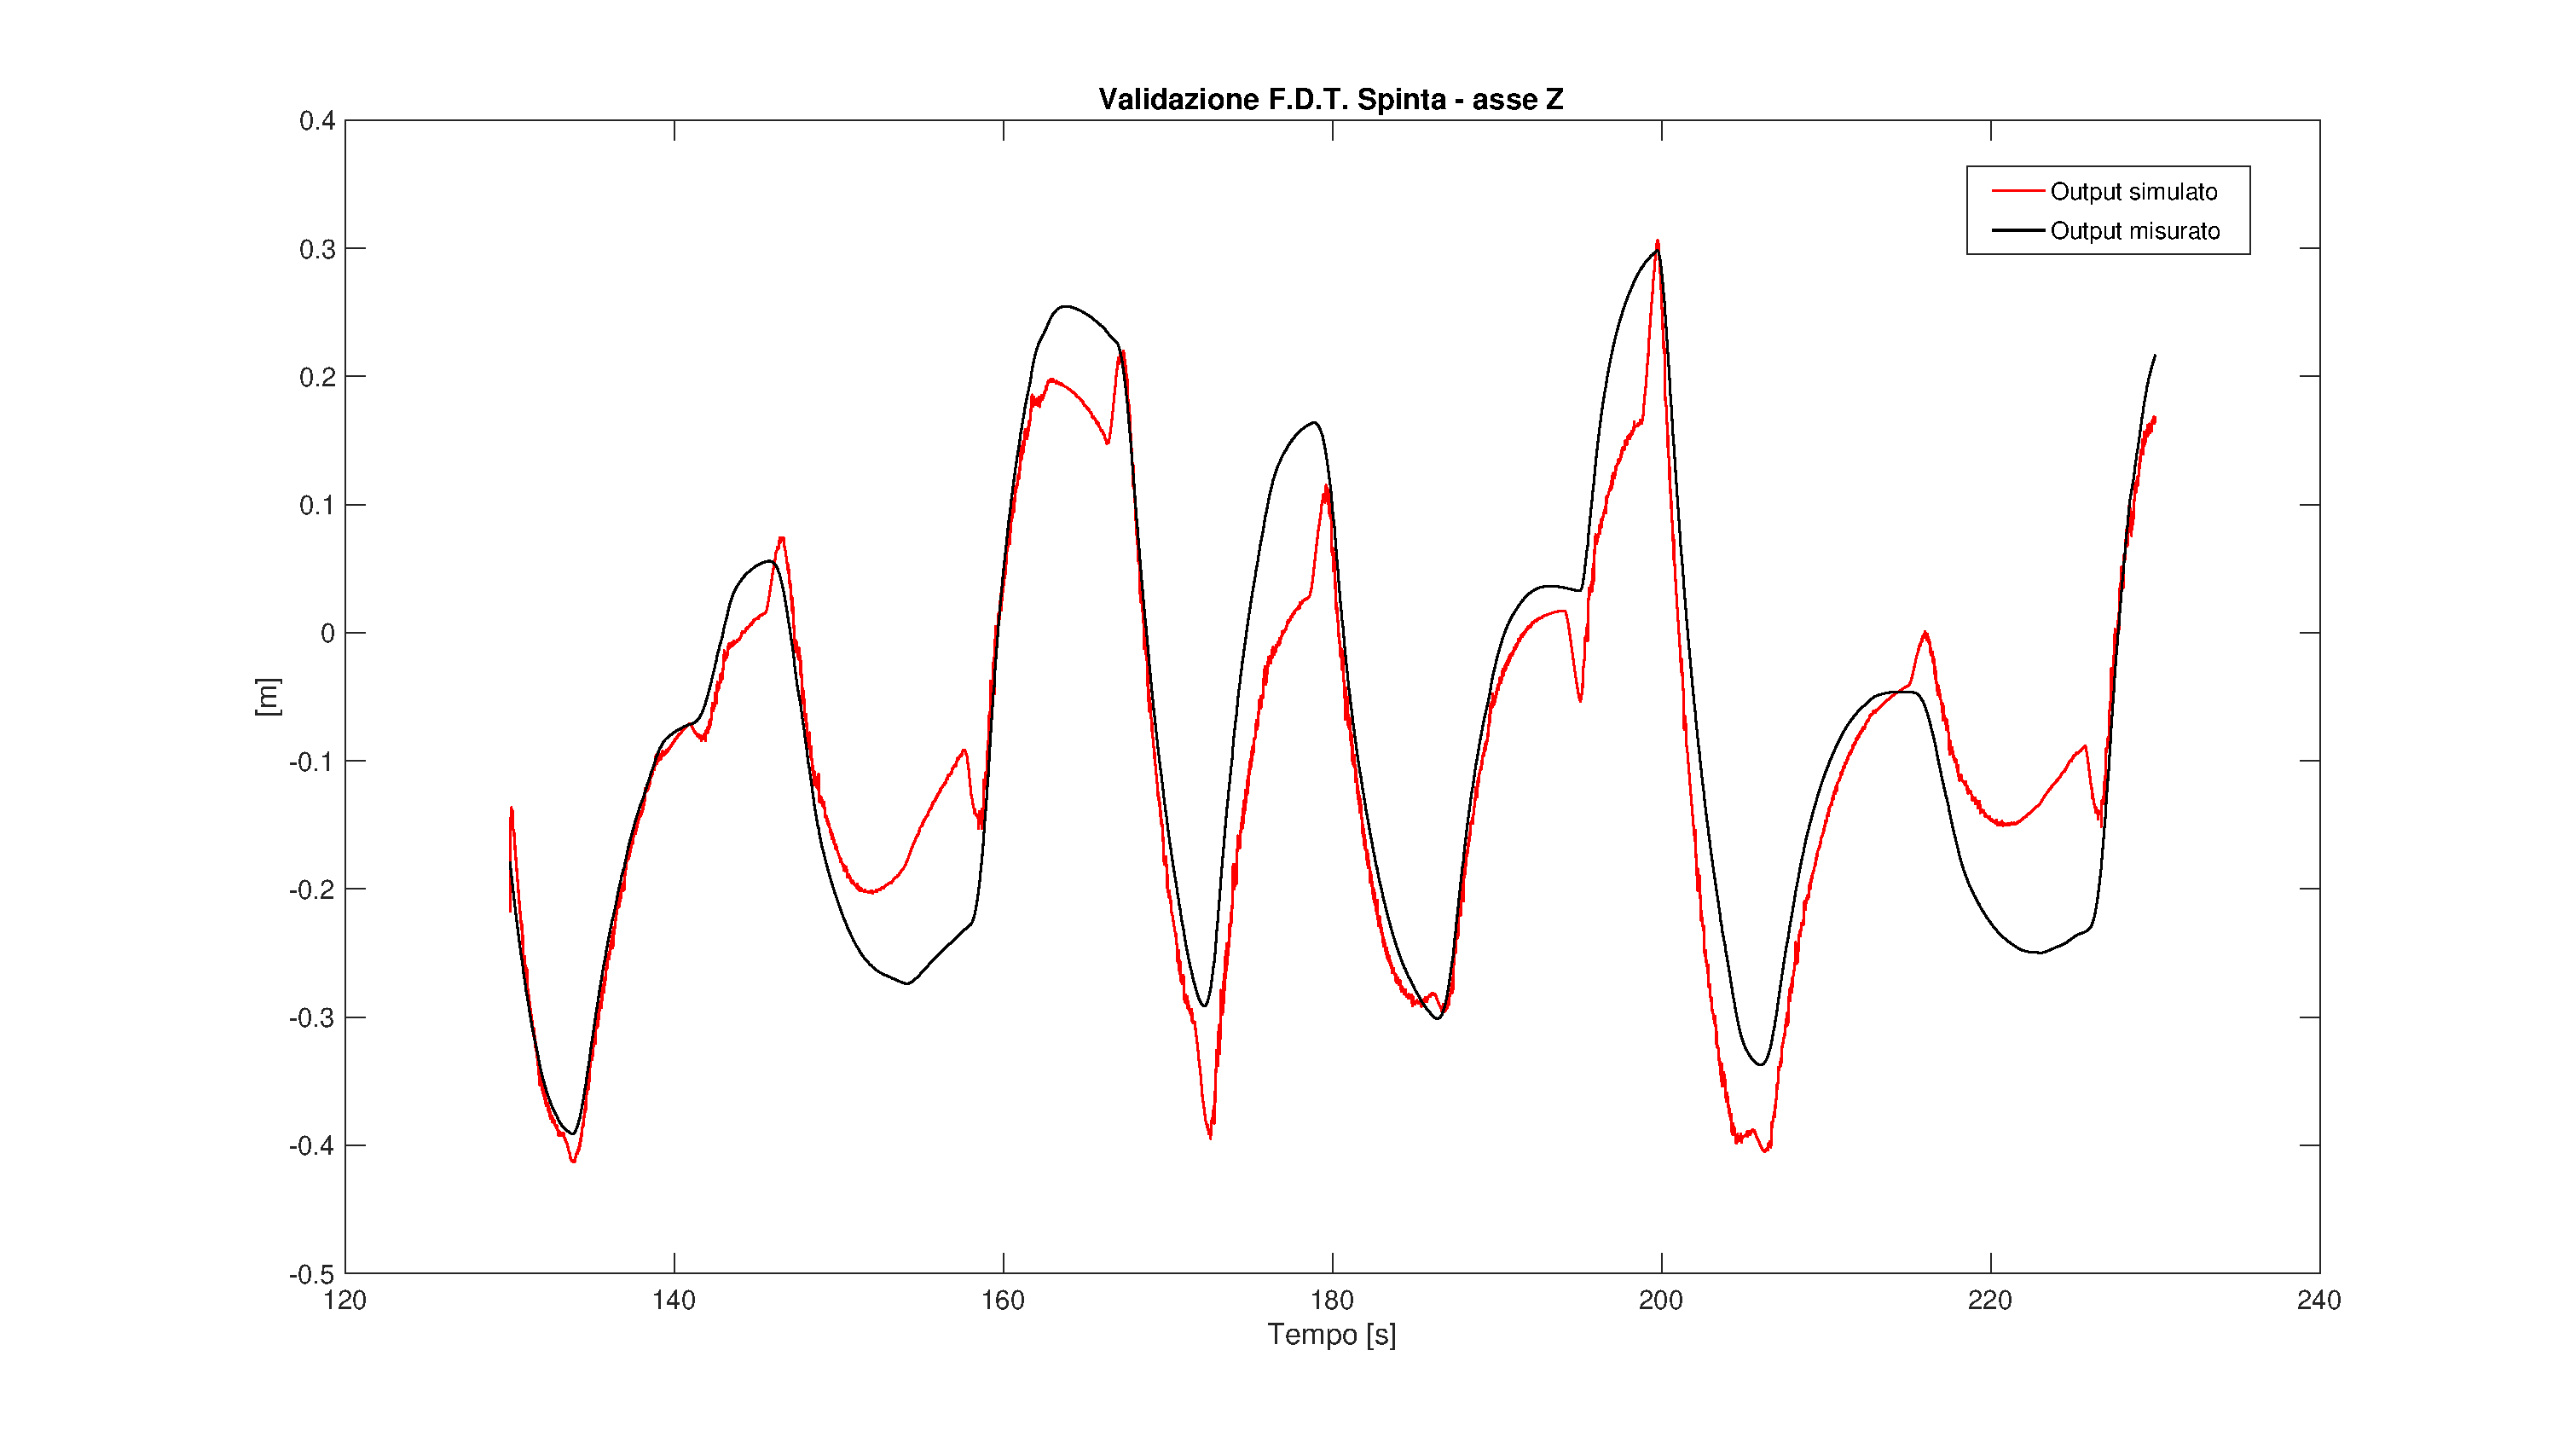
\includegraphics[width=1\textwidth]{gfx/SysId/tzmodel}
	\caption[Validazione F.D.T. Spinta e posizione lungo Z.]{Validazione F.D.T. tra spinta e posizione lungo Z.}
	\label{fig:tz_model}
\end{figure}

Si noti che nella validazione dei modelli è stato riportato il segnale in uscita (e la risposta del modello identificato) ristretto ad un preciso intervallo di tempo. Tale intervallo è stato scelto in modo tale da ottenere la migliore compatibilità del modello con i dati registrati.

\pagebreak

\subsection{Analisi in Frequenza}
In questa sezione si discutono e confrontano le risposte in frequenza relative alle tre funzioni di trasferimento identificate.\\

Come mostra Figura \ref{fig:tz_freq} e come si nota dalla funzione di trasferimento $W_Z(s)$ definita nella \ref{fdtZ}, la risposta del quadrirotore lungo l'asse verticale è asintoticamente stabile e non oscillatoria, essendo caratterizzata esclusivamente da poli reali situati nel semiasse negativo.

\begin{figure}[H]
	\centering
	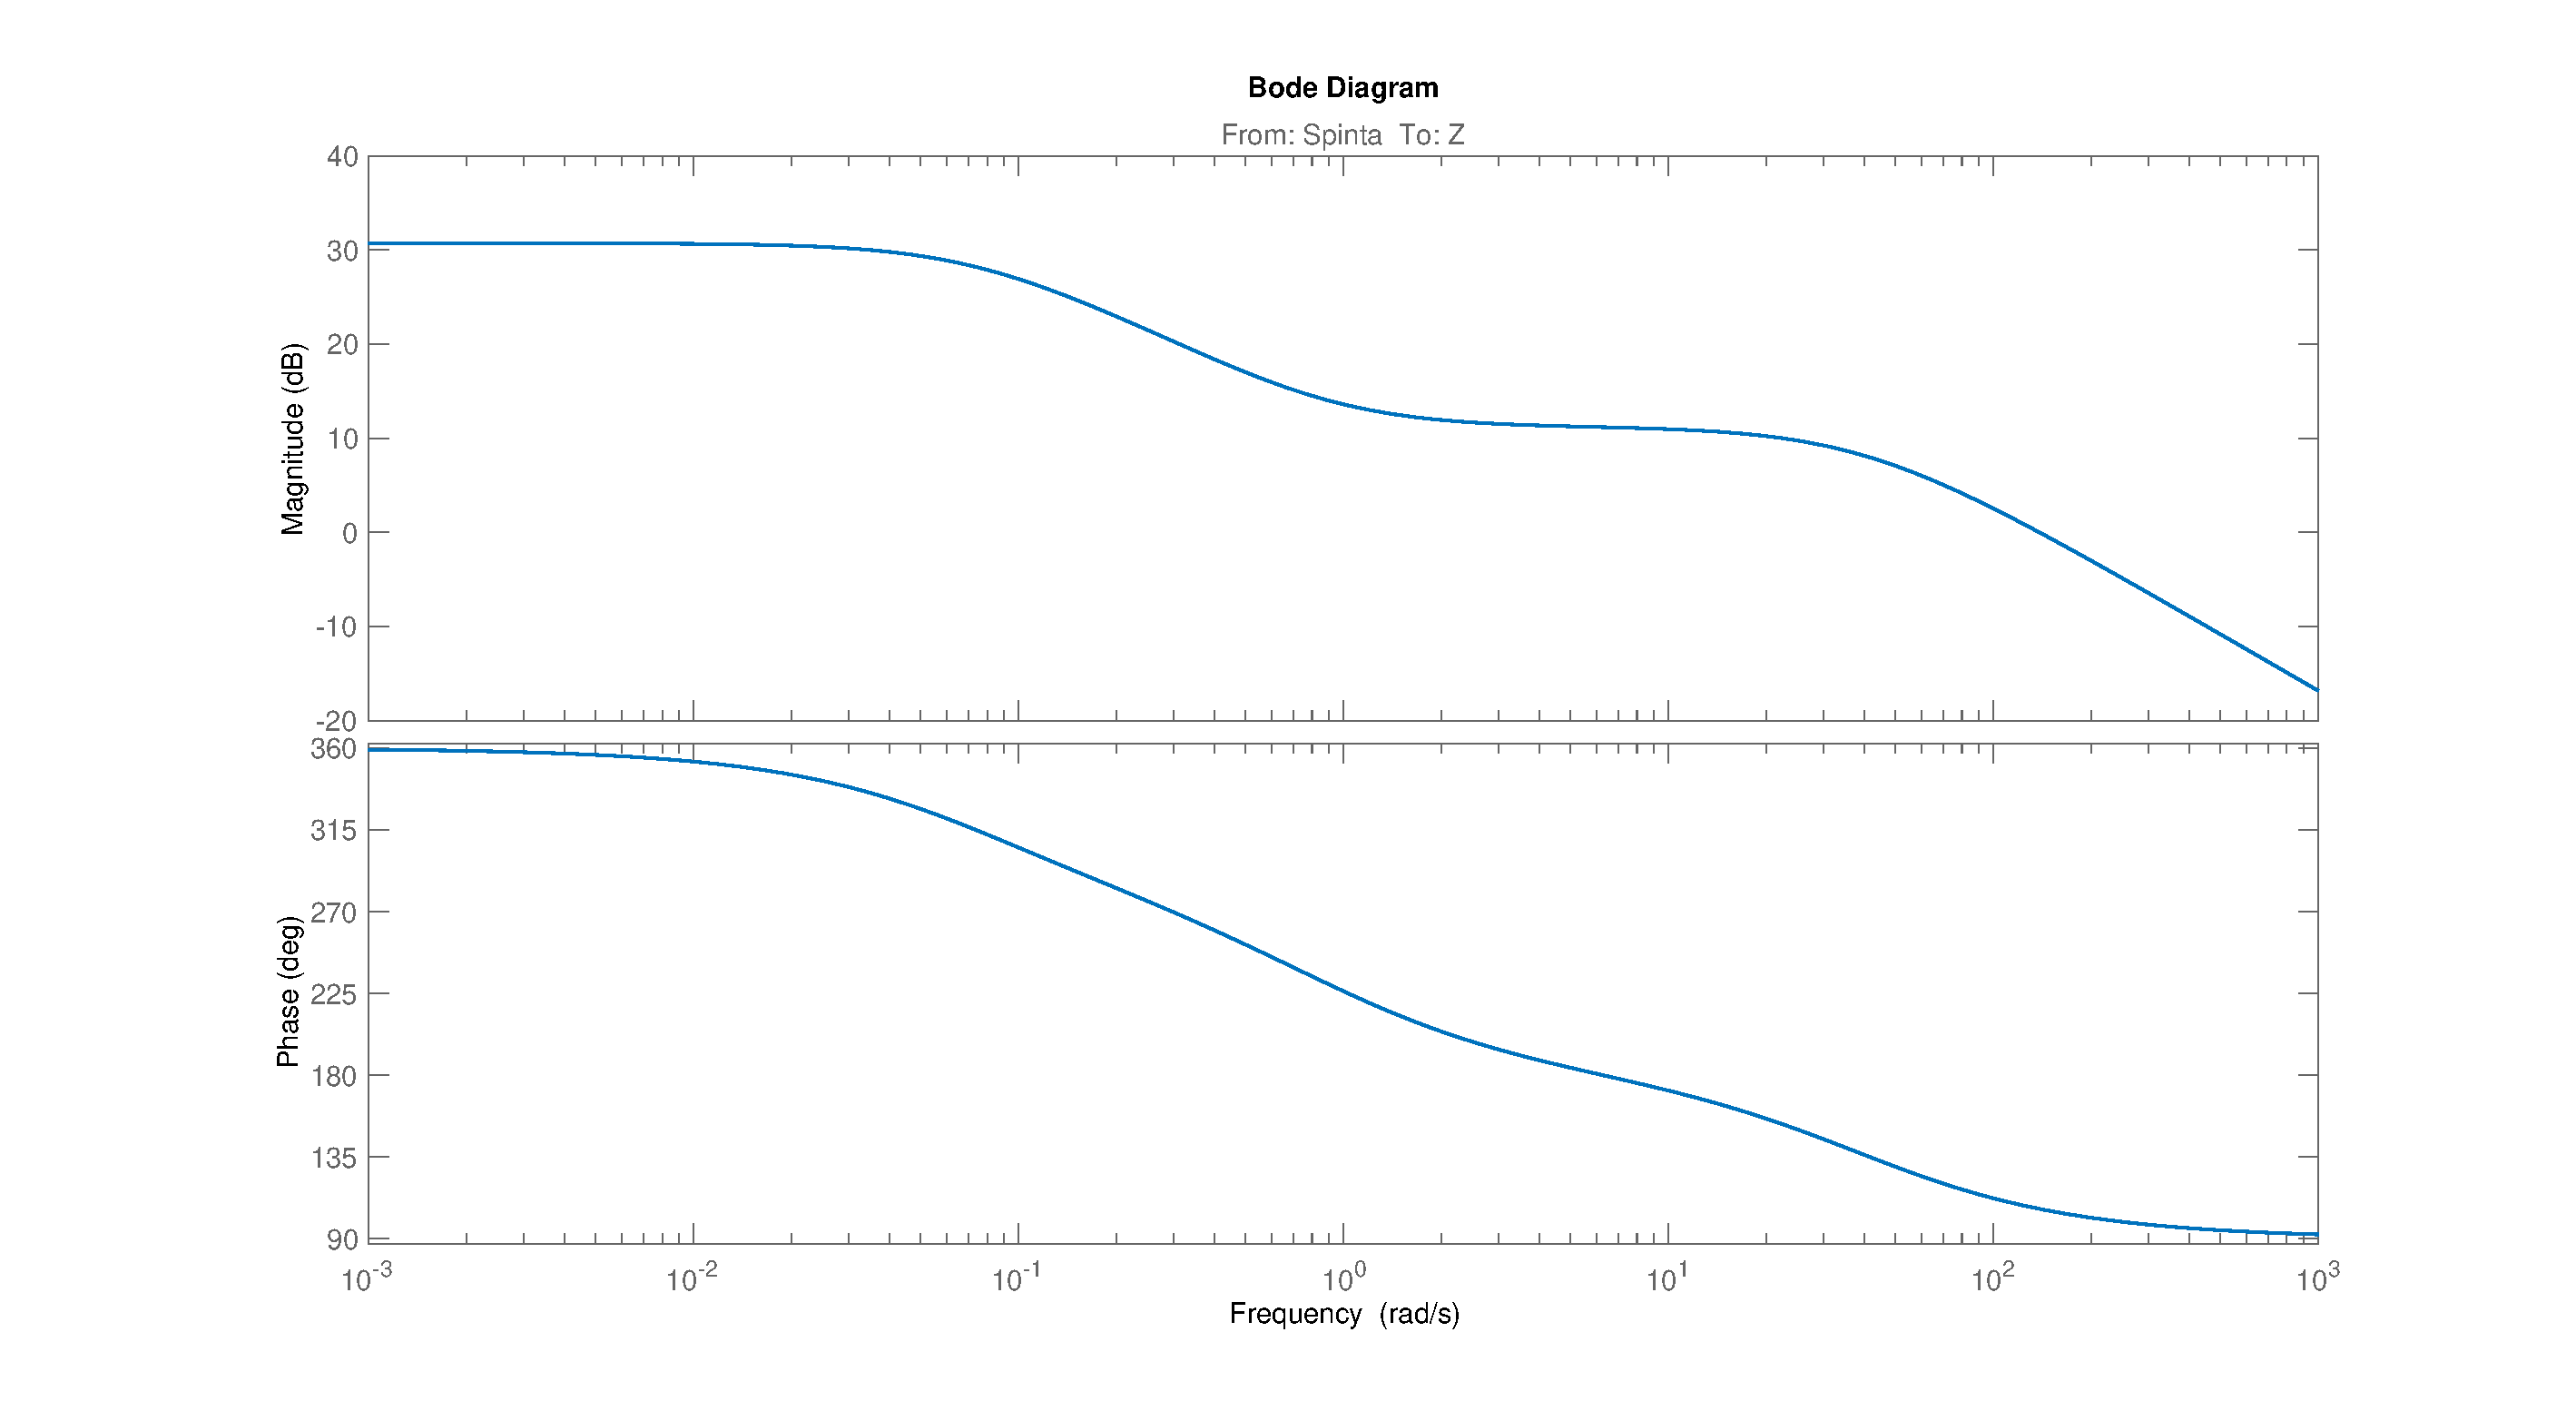
\includegraphics[width=1\textwidth]{gfx/SysId/tzbode}
	\caption[Diagrammi di Bode F.D.T. Spinta e posizione lungo Z.]{Diagrammi di Bode (modulo e fase) della F.D.T. tra spinta e posizione lungo Z.}
	\label{fig:tz_freq}
\end{figure}

D'altra parte, non sorprendentemente, le risposte in frequenza relative all'asse laterale e longitudinale (rispettivamente Figura \ref{fig:ry_freq} e Figura \ref{fig:px_freq}) sono instabili (poli a parte reale positiva) e caratterizzate da modi oscillatori (poli complessi e coniugati). Inoltre, c'è una forte simmetria tra questi due modelli. In particolare, osservando le funzioni di trasferimento $W_X(s)$ e $W_Z(s)$ definite dalle equazioni \ref{fdtX} e \ref{fdtZ}, si nota una simile dislocazione di poli e zeri nel piano complesso e questo denota che il modello identificato è preciso abbastanza da aver catturato la forte simmetria del quadrirotore.

\begin{figure}[H]
	\centering
	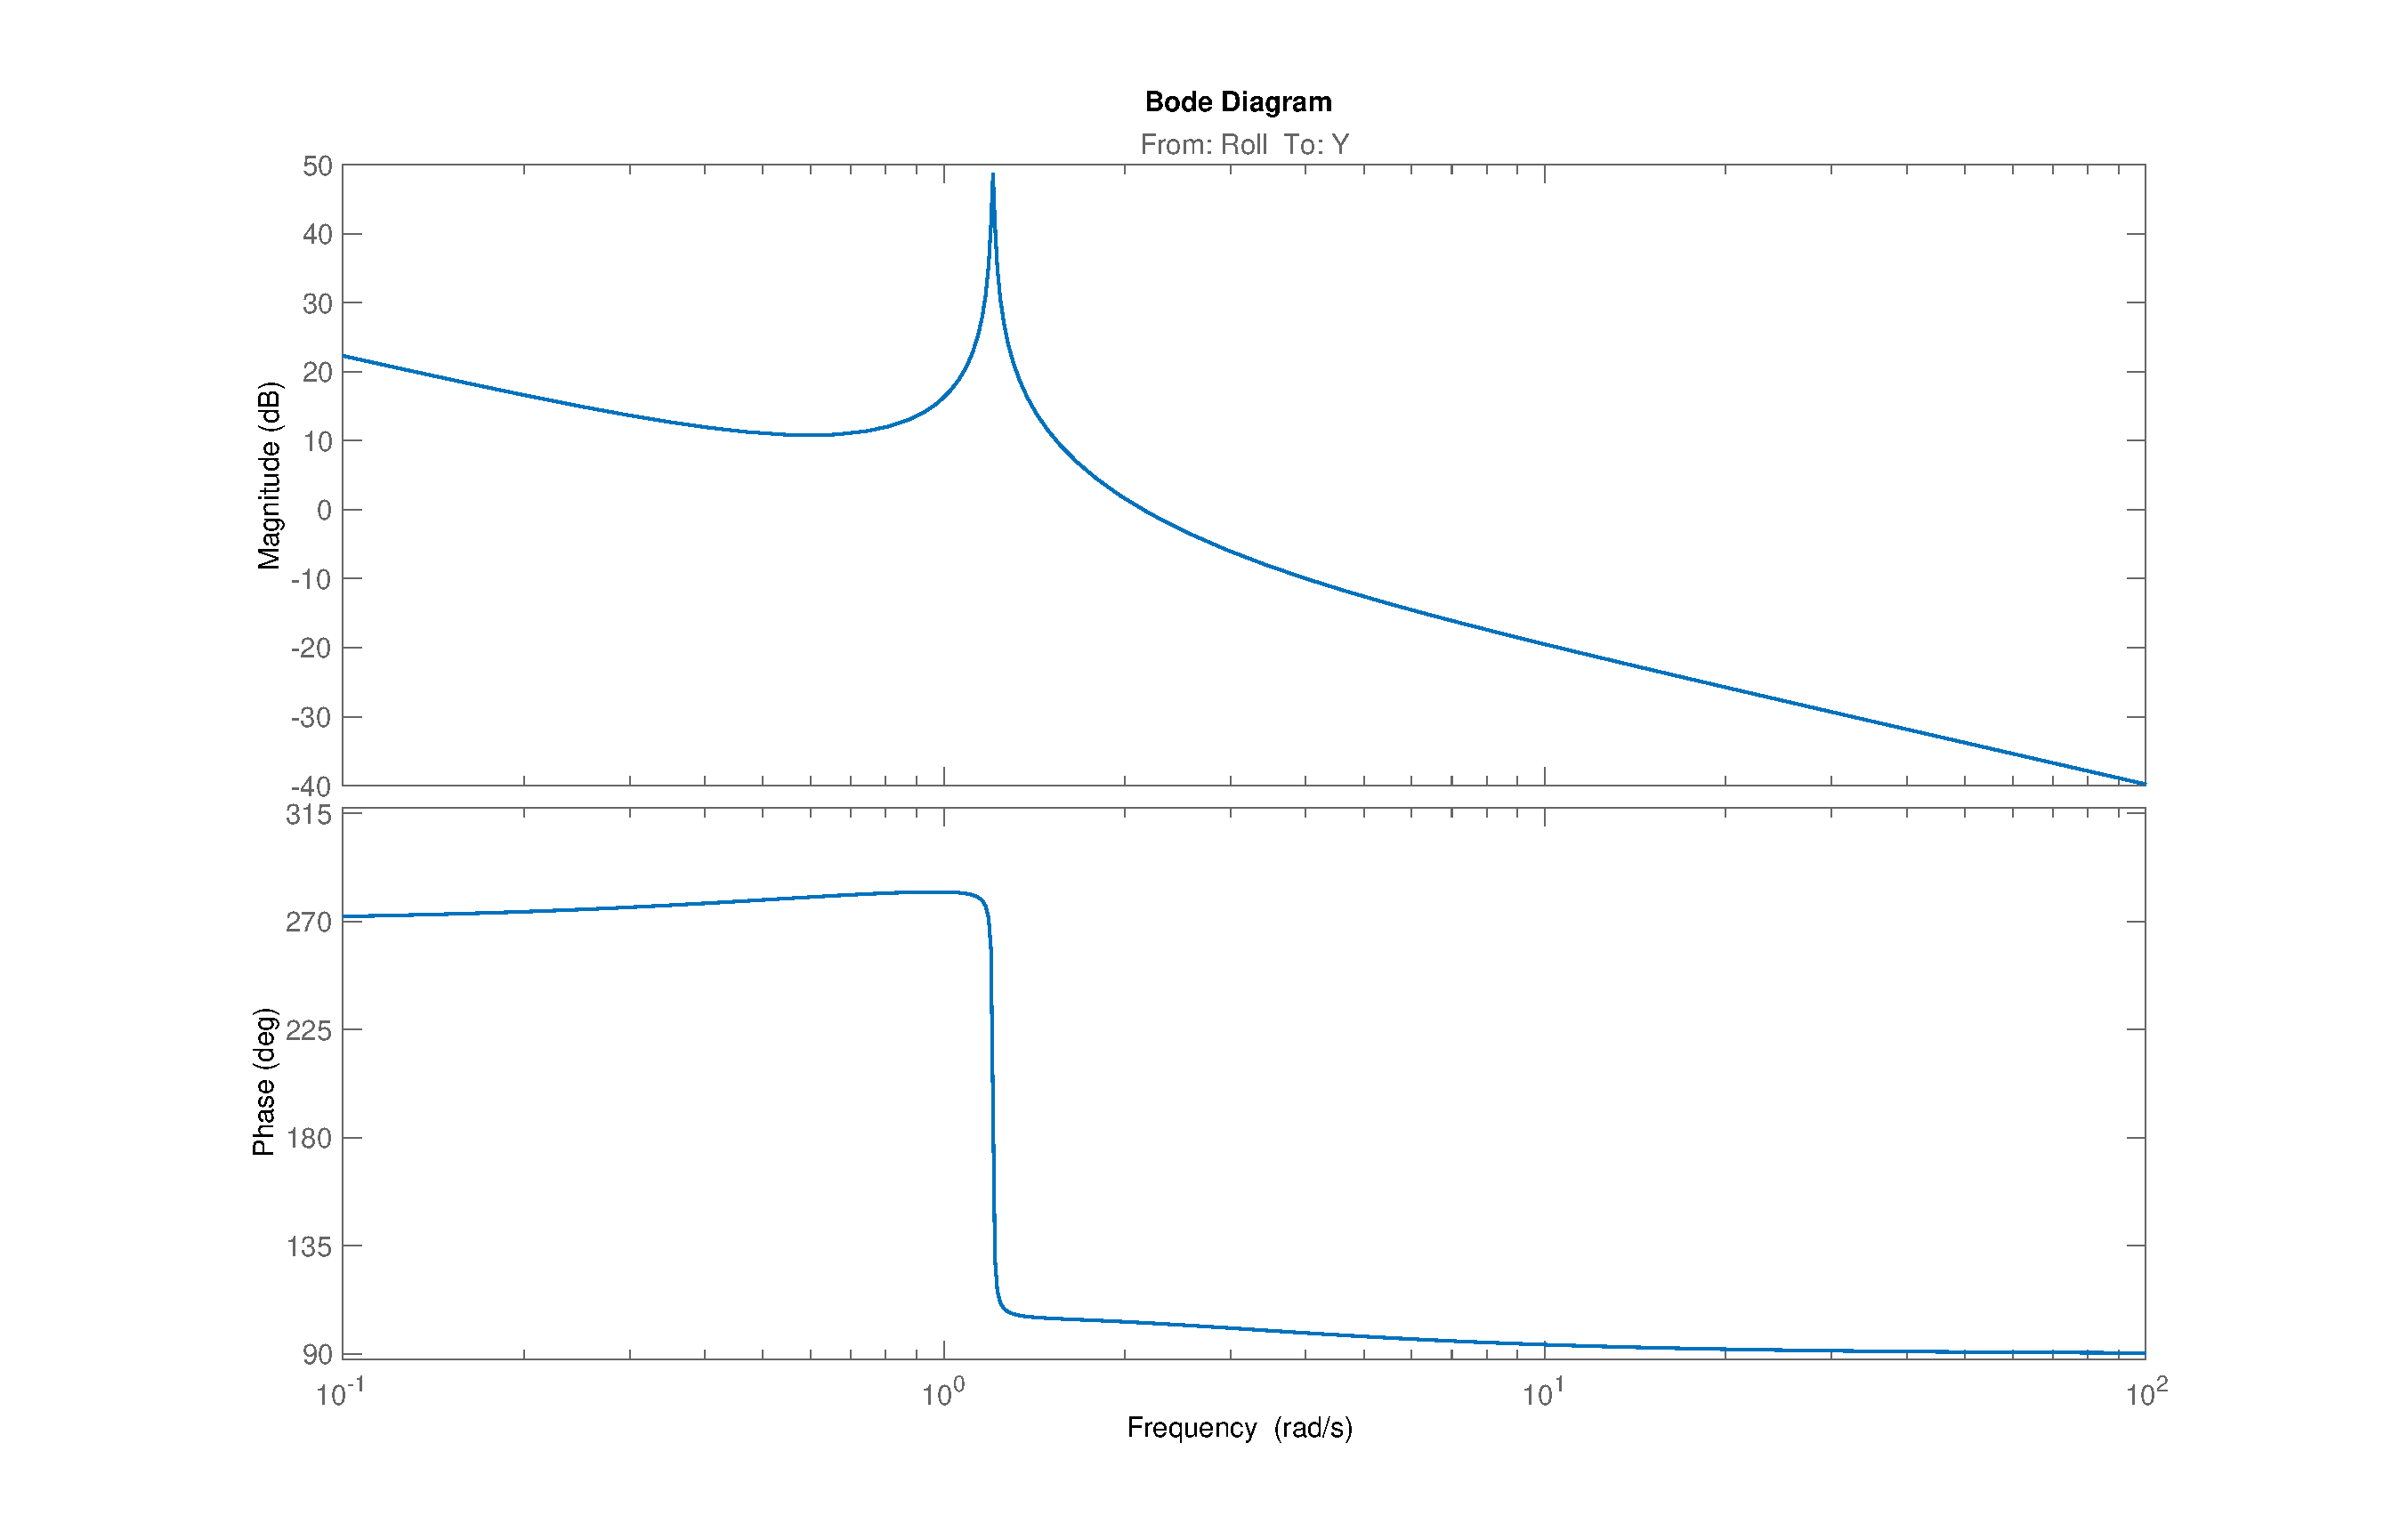
\includegraphics[width=1\textwidth]{gfx/SysId/rybode}
	\caption[Diagrammi di Bode F.D.T. Rollio e posizione lungo Y.]{Diagrammi di Bode (modulo e fase) della F.D.T. tra rollio e posizione lungo Y.}
	\label{fig:ry_freq}
\end{figure}

A causa delle limitazioni nella durata degli esperimenti e dell'azione a bassa frequenza del controllore in retroazione, che maschera la vera dinamica del sistema, ci si aspetta una significativa incertezza nella parte a bassa frequenza delle risposte dei modelli \acs{SISO} identificati. Questo si verifica maggiormente nei due modelli relativi agli spostamenti del drone nel piano XY (roll e pitch), essendo modelli instabili. Il modello lungo l'asse Z, infatti, essendo stabile, potrebbe anche essere simulato a ciclo aperto e non risentirebbe affatto dell'azione del controllore a bassa frequenza.\\

Ad ogni modo, quest'ultima problematica non è così importante dato il modello identificato è principalmente destinato alla progettazione di leggi di controllo. Quindi, è fondamentale avere un modello accurato introno alla frequenza di taglio, ma si può accettare un certo grado di incertezza a basse (e alte) frequenze.

\begin{figure}[H]
	\centering
	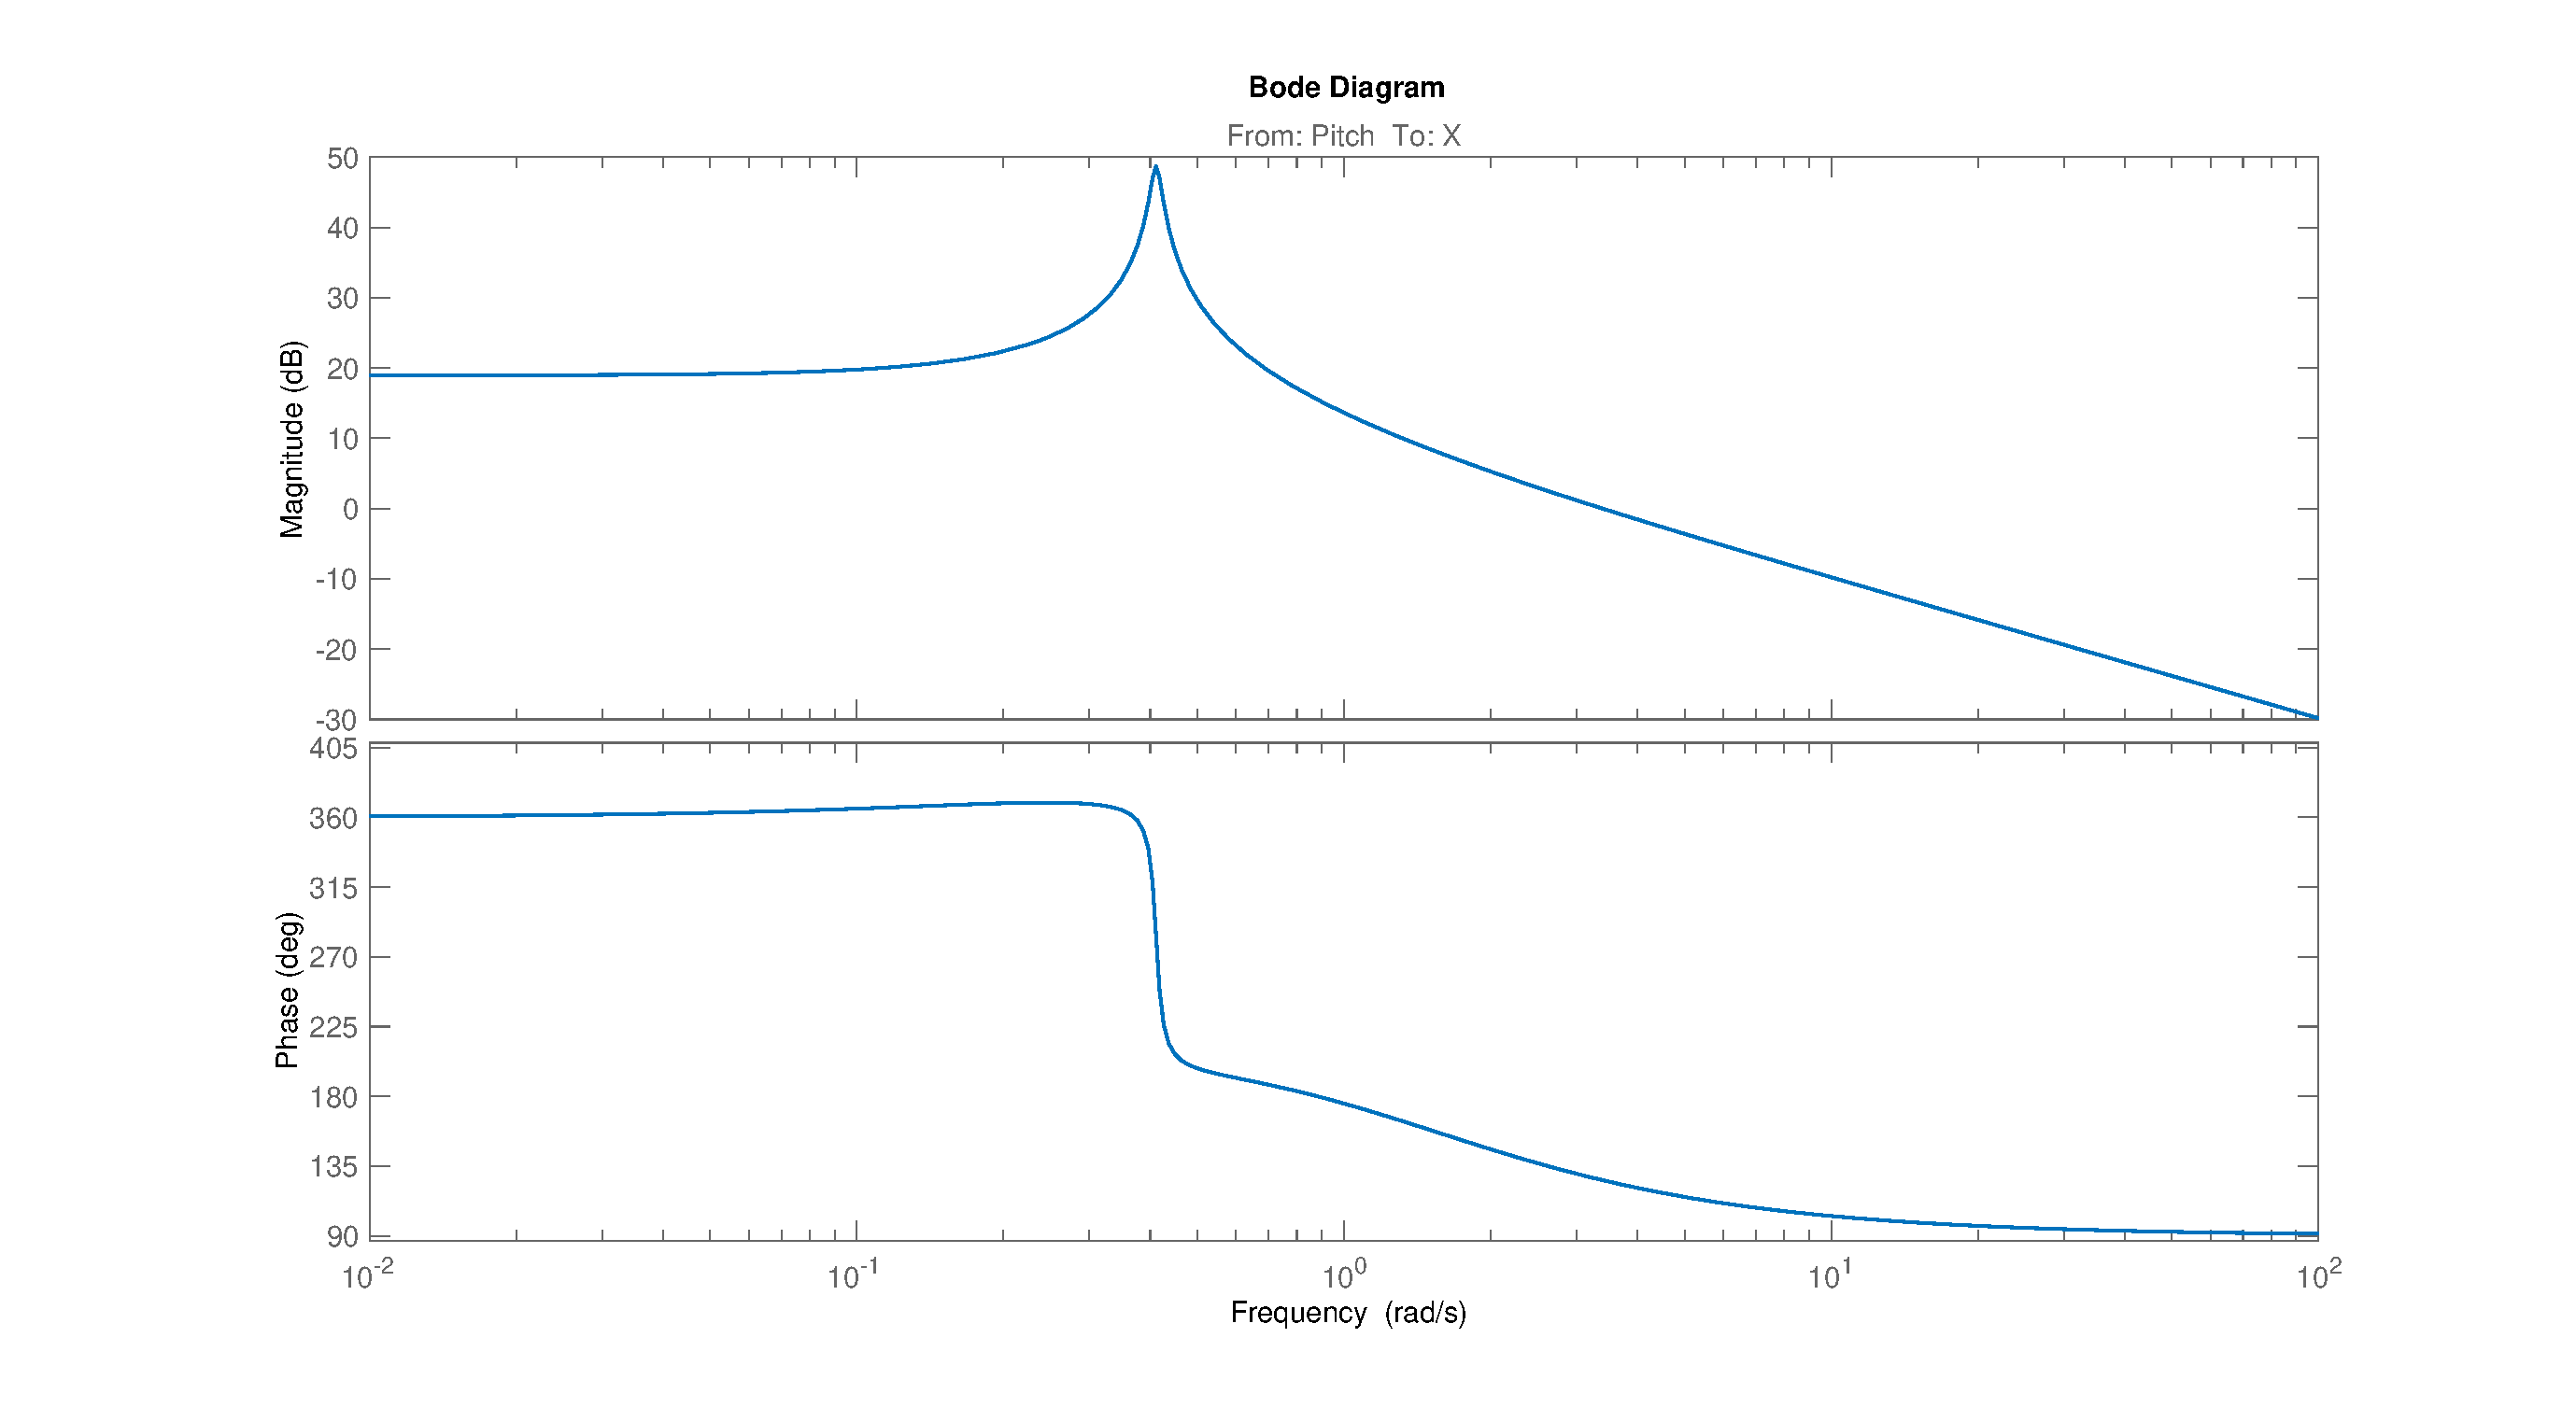
\includegraphics[width=1\textwidth]{gfx/SysId/pxbode}
	\caption[Diagrammi di Bode F.D.T. Beccheggio e posizione lungo X.]{Diagrammi di Bode (modulo e fase) della F.D.T. tra beccheggio e posizione lungo X.}
	\label{fig:px_freq}
\end{figure}
